\documentclass[]{book}
\usepackage{lmodern}
\usepackage{amssymb,amsmath}
\usepackage{ifxetex,ifluatex}
\usepackage{fixltx2e} % provides \textsubscript
\ifnum 0\ifxetex 1\fi\ifluatex 1\fi=0 % if pdftex
  \usepackage[T1]{fontenc}
  \usepackage[utf8]{inputenc}
\else % if luatex or xelatex
  \ifxetex
    \usepackage{mathspec}
  \else
    \usepackage{fontspec}
  \fi
  \defaultfontfeatures{Ligatures=TeX,Scale=MatchLowercase}
  \newcommand{\euro}{€}
\fi
% use upquote if available, for straight quotes in verbatim environments
\IfFileExists{upquote.sty}{\usepackage{upquote}}{}
% use microtype if available
\IfFileExists{microtype.sty}{%
\usepackage{microtype}
\UseMicrotypeSet[protrusion]{basicmath} % disable protrusion for tt fonts
}{}
\usepackage[margin=1in]{geometry}
\usepackage{hyperref}
\PassOptionsToPackage{usenames,dvipsnames}{color} % color is loaded by hyperref
\hypersetup{unicode=true,
            pdftitle={Advanced Visualisation and Data Wrangling in R},
            pdfauthor={TJ McKinley},
            colorlinks=true,
            linkcolor=blue,
            citecolor=Blue,
            urlcolor=Blue,
            breaklinks=true}
\urlstyle{same}  % don't use monospace font for urls
\usepackage{color}
\usepackage{fancyvrb}
\newcommand{\VerbBar}{|}
\newcommand{\VERB}{\Verb[commandchars=\\\{\}]}
\DefineVerbatimEnvironment{Highlighting}{Verbatim}{commandchars=\\\{\}}
% Add ',fontsize=\small' for more characters per line
\usepackage{framed}
\definecolor{shadecolor}{RGB}{248,248,248}
\newenvironment{Shaded}{\begin{snugshade}}{\end{snugshade}}
\newcommand{\KeywordTok}[1]{\textcolor[rgb]{0.13,0.29,0.53}{\textbf{{#1}}}}
\newcommand{\DataTypeTok}[1]{\textcolor[rgb]{0.13,0.29,0.53}{{#1}}}
\newcommand{\DecValTok}[1]{\textcolor[rgb]{0.00,0.00,0.81}{{#1}}}
\newcommand{\BaseNTok}[1]{\textcolor[rgb]{0.00,0.00,0.81}{{#1}}}
\newcommand{\FloatTok}[1]{\textcolor[rgb]{0.00,0.00,0.81}{{#1}}}
\newcommand{\ConstantTok}[1]{\textcolor[rgb]{0.00,0.00,0.00}{{#1}}}
\newcommand{\CharTok}[1]{\textcolor[rgb]{0.31,0.60,0.02}{{#1}}}
\newcommand{\SpecialCharTok}[1]{\textcolor[rgb]{0.00,0.00,0.00}{{#1}}}
\newcommand{\StringTok}[1]{\textcolor[rgb]{0.31,0.60,0.02}{{#1}}}
\newcommand{\VerbatimStringTok}[1]{\textcolor[rgb]{0.31,0.60,0.02}{{#1}}}
\newcommand{\SpecialStringTok}[1]{\textcolor[rgb]{0.31,0.60,0.02}{{#1}}}
\newcommand{\ImportTok}[1]{{#1}}
\newcommand{\CommentTok}[1]{\textcolor[rgb]{0.56,0.35,0.01}{\textit{{#1}}}}
\newcommand{\DocumentationTok}[1]{\textcolor[rgb]{0.56,0.35,0.01}{\textbf{\textit{{#1}}}}}
\newcommand{\AnnotationTok}[1]{\textcolor[rgb]{0.56,0.35,0.01}{\textbf{\textit{{#1}}}}}
\newcommand{\CommentVarTok}[1]{\textcolor[rgb]{0.56,0.35,0.01}{\textbf{\textit{{#1}}}}}
\newcommand{\OtherTok}[1]{\textcolor[rgb]{0.56,0.35,0.01}{{#1}}}
\newcommand{\FunctionTok}[1]{\textcolor[rgb]{0.00,0.00,0.00}{{#1}}}
\newcommand{\VariableTok}[1]{\textcolor[rgb]{0.00,0.00,0.00}{{#1}}}
\newcommand{\ControlFlowTok}[1]{\textcolor[rgb]{0.13,0.29,0.53}{\textbf{{#1}}}}
\newcommand{\OperatorTok}[1]{\textcolor[rgb]{0.81,0.36,0.00}{\textbf{{#1}}}}
\newcommand{\BuiltInTok}[1]{{#1}}
\newcommand{\ExtensionTok}[1]{{#1}}
\newcommand{\PreprocessorTok}[1]{\textcolor[rgb]{0.56,0.35,0.01}{\textit{{#1}}}}
\newcommand{\AttributeTok}[1]{\textcolor[rgb]{0.77,0.63,0.00}{{#1}}}
\newcommand{\RegionMarkerTok}[1]{{#1}}
\newcommand{\InformationTok}[1]{\textcolor[rgb]{0.56,0.35,0.01}{\textbf{\textit{{#1}}}}}
\newcommand{\WarningTok}[1]{\textcolor[rgb]{0.56,0.35,0.01}{\textbf{\textit{{#1}}}}}
\newcommand{\AlertTok}[1]{\textcolor[rgb]{0.94,0.16,0.16}{{#1}}}
\newcommand{\ErrorTok}[1]{\textcolor[rgb]{0.64,0.00,0.00}{\textbf{{#1}}}}
\newcommand{\NormalTok}[1]{{#1}}
\usepackage{longtable,booktabs}
\usepackage{graphicx,grffile}
\makeatletter
\def\maxwidth{\ifdim\Gin@nat@width>\linewidth\linewidth\else\Gin@nat@width\fi}
\def\maxheight{\ifdim\Gin@nat@height>\textheight\textheight\else\Gin@nat@height\fi}
\makeatother
% Scale images if necessary, so that they will not overflow the page
% margins by default, and it is still possible to overwrite the defaults
% using explicit options in \includegraphics[width, height, ...]{}
\setkeys{Gin}{width=\maxwidth,height=\maxheight,keepaspectratio}
\setlength{\parindent}{0pt}
\setlength{\parskip}{6pt plus 2pt minus 1pt}
\setlength{\emergencystretch}{3em}  % prevent overfull lines
\providecommand{\tightlist}{%
  \setlength{\itemsep}{0pt}\setlength{\parskip}{0pt}}
\setcounter{secnumdepth}{5}

%%% Use protect on footnotes to avoid problems with footnotes in titles
\let\rmarkdownfootnote\footnote%
\def\footnote{\protect\rmarkdownfootnote}

%%% Change title format to be more compact
\usepackage{titling}

% Create subtitle command for use in maketitle
\newcommand{\subtitle}[1]{
  \posttitle{
    \begin{center}\large#1\end{center}
    }
}

\setlength{\droptitle}{-2em}

  \title{Advanced Visualisation and Data Wrangling in R}
    \pretitle{\vspace{\droptitle}\centering\huge}
  \posttitle{\par}
    \author{TJ McKinley}
    \preauthor{\centering\large\emph}
  \postauthor{\par}
    \date{}
    \predate{}\postdate{}
  

% Redefines (sub)paragraphs to behave more like sections
\ifx\paragraph\undefined\else
\let\oldparagraph\paragraph
\renewcommand{\paragraph}[1]{\oldparagraph{#1}\mbox{}}
\fi
\ifx\subparagraph\undefined\else
\let\oldsubparagraph\subparagraph
\renewcommand{\subparagraph}[1]{\oldsubparagraph{#1}\mbox{}}
\fi

% latex macro to create task boxes
\usepackage{tcolorbox}

\definecolor{taskCol}{HTML}{404040}
\definecolor{taskCol1}{HTML}{808080}

\tcbset{colback=white,colframe=taskCol,arc=0mm}

%trick to fool markdown into compiling
\newcommand{\bblockT}[1]{\begin{tcolorbox}[title = Task #1]}
\newcommand{\eblockT}{\end{tcolorbox}}
\newcommand{\bblockS}[1]{\begin{tcolorbox}[title = Solution #1, colframe=taskCol1]}
\newcommand{\eblockS}{\end{tcolorbox}}

%set solution button link
\usepackage{tikz}

\newcommand{\buttonT}[1]{
    \begin{tikzpicture}
    \node[
        inner sep=5pt,
        draw=taskCol,
        fill=taskCol,
        rounded corners=2pt,
        text=white
    ] (c1) {#1};
    \end{tikzpicture}
}

\newcommand{\buttonS}[1]{
    \begin{tikzpicture}
    \node[
        inner sep=5pt,
        draw=taskCol1,
        fill=taskCol1,
        rounded corners=2pt,
        text=white
    ] (c1) {#1};
    \end{tikzpicture}
}

\usepackage{amsthm}
\newtheorem{theorem}{Theorem}[chapter]
\newtheorem{lemma}{Lemma}[chapter]
\theoremstyle{definition}
\newtheorem{definition}{Definition}[chapter]
\newtheorem{corollary}{Corollary}[chapter]
\newtheorem{proposition}{Proposition}[chapter]
\theoremstyle{definition}
\newtheorem{example}{Example}[chapter]
\theoremstyle{definition}
\newtheorem{exercise}{Exercise}[chapter]
\theoremstyle{remark}
\newtheorem*{remark}{Remark}
\newtheorem*{solution}{Solution}
\begin{document}
\maketitle

{
\hypersetup{linkcolor=black}
\setcounter{tocdepth}{1}
\tableofcontents
}
\chapter*{Introduction}\label{introduction}
\addcontentsline{toc}{chapter}{Introduction}

In this workshop we will introduce some R packages that provide really
useful and powerful functions for doing visualisation of complex data
sets. We will see how R can be used to make informative animations, and
even interactive HTML graphics.

\section*{Tasks}\label{tasks}
\addcontentsline{toc}{section}{Tasks}

\hypertarget{tsk1}{}\bblockT{1}

All \textbf{tasks} will be denoted in panel boxes like this one. In the
HTML version, all solutions can be toggled by hitting the \textbf{Show
Solution} buttons. In the PDF version solutions are given in the
Appendix and are linked via the \textbf{Show Solution} buttons. \eblockT

\hyperlink{sol1}{\buttonS{Show Solution}}

\chapter{Advanced Visualisation}\label{advanced-visualisation}

In the next couple of practicals we will introduce you to some really
useful packages for data wrangling and visualisation: notably
\href{https://cran.r-project.org/web/packages/tidyr/}{\texttt{tidyr}},
\href{https://cran.r-project.org/web/packages/dplyr/index.html}{\texttt{dplyr}}
and
\href{https://cran.r-project.org/web/packages/ggplot2/index.html}{\texttt{ggplot2}}.
We start with a motivating example.

\section{Gapminder}\label{gapminder}

\href{https://en.wikipedia.org/wiki/Hans_Rosling}{Professor Hans
Rosling} has made a name for himself in the field of data visualisation
with his groundbreaking \href{https://www.gapminder.org/}{Gapminder}
project.

\begin{center}\includegraphics{images/hans} \end{center}

For a slightly longer presentation, his TED talk on global development
has been watched over 11 million times. If you have 20 minutes, it can
be found
\href{https://www.ted.com/talks/hans_rosling_shows_the_best_stats_you_ve_ever_seen?utm_source=tedcomshare\&utm_medium=referral\&utm_campaign=tedspread}{here},
and is well worth a watch!

\begin{quote}
\textbf{Update}: More-or-less as I finished these practical notes, the
news broke that Professor Rosling had sadly passed away on 7th February
2017, aged 68. I hope you will find some time to explore the
\href{https://www.gapminder.org/}{Gapminder} website, and appreciate the
contribution that he made to the world of public health and education.
He presented a world-view based on facts and data; to this end he
provided innovative and fascinating ways to explore and understand data,
disseminated these findings with pathos and humour, and used this
information to challenge many of our pre-conceptions about public health
and the developing world. An obituary from the Guardian can be found
\href{https://www.theguardian.com/global-development/2017/feb/07/hans-rosling-obituary}{here}.
\end{quote}

The \href{https://www.gapminder.org/}{Gapminder} website provides really
informative interactive visualisations for many fascinating data sets.
In this pracical we will explore how to use R to try to recreate
something similar to the types of visualisation that Gapminder provides,
and see how high-end R packages have been developed that provide a
systematic and flexible way to generate complex plots / visualisations
from data. We will begin by trying to emulate the plot in Figure
\ref{fig:gapminder}.

We will do this first by using R's base graphics system, before
introducing a set of functions from a powerful package called
\href{https://cran.r-project.org/web/packages/ggplot2/index.html}{\texttt{ggplot2}}.

\subsection{Gapminder data}\label{gapminder-data}

Datasets from the Gapminder project can be downloaded from
\url{https://www.gapminder.org/data}. However, this particular data set
is available in a package in R called (naturally)
\href{https://cran.r-project.org/web/packages/gapminder/index.html}{\texttt{gapminder}}.
This can be installed in the usual way. (For ease later on, make sure
the \texttt{tidyr}, \texttt{dplyr} and \texttt{ggplot2} packages are
also installed.)

\begin{Shaded}
\begin{Highlighting}[]
\KeywordTok{install.packages}\NormalTok{(}\StringTok{"gapminder"}\NormalTok{)}
\KeywordTok{install.packages}\NormalTok{(}\StringTok{"tidyr"}\NormalTok{)}
\KeywordTok{install.packages}\NormalTok{(}\StringTok{"tibble"}\NormalTok{)}
\KeywordTok{install.packages}\NormalTok{(}\StringTok{"dplyr"}\NormalTok{)}
\KeywordTok{install.packages}\NormalTok{(}\StringTok{"ggplot2"}\NormalTok{)}
\end{Highlighting}
\end{Shaded}

Once you have it installed we need to load the packages.

\begin{Shaded}
\begin{Highlighting}[]
\KeywordTok{library}\NormalTok{(gapminder)}
\KeywordTok{library}\NormalTok{(tidyr)}
\KeywordTok{library}\NormalTok{(tibble)}
\end{Highlighting}
\end{Shaded}

\begin{quote}
Two really useful cheat sheets to have for data wrangling can be found
\href{https://www.rstudio.com/resources/cheatsheets/}{here}, under
\href{https://github.com/rstudio/cheatsheets/raw/master/source/pdfs/data-import-cheatsheet.pdf}{Data
Import Cheat Sheet} and
\href{https://github.com/rstudio/cheatsheets/raw/master/source/pdfs/data-transformation-cheatsheet.pdf}{Data
Transformation Cheat Sheet}.
\end{quote}

To have a quick look at the data, which are available as an object
called \texttt{gapminder}. We can use the \texttt{head()} and
\texttt{tail()} functions, which print the top and bottom of a data
frame respectively. The functions \texttt{dim()} and \texttt{summary()}
are also useful e.g.

\begin{Shaded}
\begin{Highlighting}[]
\KeywordTok{dim}\NormalTok{(gapminder)}
\end{Highlighting}
\end{Shaded}

\begin{verbatim}
## [1] 1704    6
\end{verbatim}

\begin{Shaded}
\begin{Highlighting}[]
\KeywordTok{head}\NormalTok{(gapminder)}
\end{Highlighting}
\end{Shaded}

\begin{verbatim}
## # A tibble: 6 x 6
##   country     continent  year lifeExp      pop gdpPercap
##   <fct>       <fct>     <int>   <dbl>    <int>     <dbl>
## 1 Afghanistan Asia       1952    28.8  8425333      779.
## 2 Afghanistan Asia       1957    30.3  9240934      821.
## 3 Afghanistan Asia       1962    32.0 10267083      853.
## 4 Afghanistan Asia       1967    34.0 11537966      836.
## 5 Afghanistan Asia       1972    36.1 13079460      740.
## 6 Afghanistan Asia       1977    38.4 14880372      786.
\end{verbatim}

\begin{Shaded}
\begin{Highlighting}[]
\KeywordTok{tail}\NormalTok{(gapminder)}
\end{Highlighting}
\end{Shaded}

\begin{verbatim}
## # A tibble: 6 x 6
##   country  continent  year lifeExp      pop gdpPercap
##   <fct>    <fct>     <int>   <dbl>    <int>     <dbl>
## 1 Zimbabwe Africa     1982    60.4  7636524      789.
## 2 Zimbabwe Africa     1987    62.4  9216418      706.
## 3 Zimbabwe Africa     1992    60.4 10704340      693.
## 4 Zimbabwe Africa     1997    46.8 11404948      792.
## 5 Zimbabwe Africa     2002    40.0 11926563      672.
## 6 Zimbabwe Africa     2007    43.5 12311143      470.
\end{verbatim}

\begin{Shaded}
\begin{Highlighting}[]
\KeywordTok{summary}\NormalTok{(gapminder)}
\end{Highlighting}
\end{Shaded}

\begin{verbatim}
##         country        continent        year         lifeExp     
##  Afghanistan:  12   Africa  :624   Min.   :1952   Min.   :23.60  
##  Albania    :  12   Americas:300   1st Qu.:1966   1st Qu.:48.20  
##  Algeria    :  12   Asia    :396   Median :1980   Median :60.71  
##  Angola     :  12   Europe  :360   Mean   :1980   Mean   :59.47  
##  Argentina  :  12   Oceania : 24   3rd Qu.:1993   3rd Qu.:70.85  
##  Australia  :  12                  Max.   :2007   Max.   :82.60  
##  (Other)    :1632                                                
##       pop              gdpPercap       
##  Min.   :6.001e+04   Min.   :   241.2  
##  1st Qu.:2.794e+06   1st Qu.:  1202.1  
##  Median :7.024e+06   Median :  3531.8  
##  Mean   :2.960e+07   Mean   :  7215.3  
##  3rd Qu.:1.959e+07   3rd Qu.:  9325.5  
##  Max.   :1.319e+09   Max.   :113523.1  
## 
\end{verbatim}

Here we can see that the data set consists of 1704 rows and 6 columns,
and contains information on country, continent, life expectancy,
population size, GDP (per capita) and year.

\begin{quote}
\textbf{Aside}: Note the slightly strange formatting when printing the
\texttt{data.frame}. This is subtly different to what you've seen
before. This is because the \texttt{gapminder} data is actually a
\texttt{tbl} object (pronounced ``tibble''), which is a special object
type. This is an enhanced \texttt{data.frame} object: \texttt{tbls} are
generally easier to examine than \texttt{data.frames}, for example they
force R to display only the data that fits onscreen. It also adds some
information about the class of each column. Try typing

\begin{Shaded}
\begin{Highlighting}[]
\NormalTok{gapminder}
\end{Highlighting}
\end{Shaded}

\begin{verbatim}
## # A tibble: 1,704 x 6
##    country     continent  year lifeExp      pop gdpPercap
##    <fct>       <fct>     <int>   <dbl>    <int>     <dbl>
##  1 Afghanistan Asia       1952    28.8  8425333      779.
##  2 Afghanistan Asia       1957    30.3  9240934      821.
##  3 Afghanistan Asia       1962    32.0 10267083      853.
##  4 Afghanistan Asia       1967    34.0 11537966      836.
##  5 Afghanistan Asia       1972    36.1 13079460      740.
##  6 Afghanistan Asia       1977    38.4 14880372      786.
##  7 Afghanistan Asia       1982    39.9 12881816      978.
##  8 Afghanistan Asia       1987    40.8 13867957      852.
##  9 Afghanistan Asia       1992    41.7 16317921      649.
## 10 Afghanistan Asia       1997    41.8 22227415      635.
## # ... with 1,694 more rows
\end{verbatim}

to see what I mean. In fact, the \texttt{tibble} package introduces the
\texttt{as\_tibble()} function to convert ordinary \texttt{data.frame}
objects to \texttt{tbls} in case you want to use this functionality in
future. Please see the
\href{https://github.com/rstudio/cheatsheets/raw/master/source/pdfs/data-import-cheatsheet.pdf}{Data
Import Cheat Sheet} for more information.

Note also that \texttt{tbl} seems to make a distinction between integers
(\texttt{\textless{}int\textgreater{}}) and doubles
(\texttt{\textless{}dbl\textgreater{}}), instead of just using
\texttt{numeric}. R makes no such distinction in practice, and so you
can think of either of these as simply \texttt{numeric} types.
\end{quote}

Let's just clarify the data:

\begin{itemize}
\tightlist
\item
  \textbf{\texttt{country}}: country of interest (\texttt{factor});
\item
  \textbf{\texttt{continent}}: continent country can be found in
  (\texttt{factor});
\item
  \textbf{\texttt{year}}: year corresponding to data (in increments of 5
  years) (\texttt{numeric});
\item
  \textbf{\texttt{lifeExp}}: life expectancy at birth (in years)
  (\texttt{numeric});
\item
  \textbf{\texttt{pop}}: population size (\texttt{numeric});
\item
  \textbf{\texttt{gdpPercap}}: GDP per capita, in dollars, by Purchasing
  Power Parities and adjusted for inflation (\texttt{numeric}).
\end{itemize}

\chapter{Visualisation (the old-fashioned
way)}\label{visualisation-the-old-fashioned-way}

R's base graphics system is very flexible, and is one of the main
reasons R has surged in popularity amongst statisticians and data
scientists. Flexibility often comes with a price, and in this case it's
that complex plotting often involves many steps. Here I will take you
through a process of building a complex plot up piece-by-piece using R's
base graphics system.

\begin{quote}
Please note there are other ways to do this, you might find a better
way!
\end{quote}

Let's start by visualising a single year, and noting that we are trying
to produce something that looks like Figure \ref{fig:gapminder}.

\begin{Shaded}
\begin{Highlighting}[]
\KeywordTok{include_graphics}\NormalTok{(}\StringTok{"images/gapminder.png"}\NormalTok{)}
\end{Highlighting}
\end{Shaded}

\begin{figure}

{\centering \includegraphics{images/gapminder} 

}

\caption{Life expectancy against GDP---screenshot from Gapminder project}\label{fig:gapminder}
\end{figure}

Let's break this plot down into various \textbf{features}:

\begin{itemize}
\tightlist
\item
  It shows data from 1952 only;
\item
  it shows a \textbf{scatterplot} of \textbf{life expectancy} on the
  \(y\)-axis, and \textbf{GDP per capita} on the \(x\)-axis;
\item
  GDP is plotted on the \textbf{\(\log_{10}\)} scale;
\item
  points are coloured according to \textbf{continent};
\item
  points are scaled according to the population of the country (more
  subtly---they are scaled according to \textbf{area}, so a point with
  \emph{double the area} of another point, has \emph{twice the
  population}).
\end{itemize}

Let's start by extracting just the subset of data from 1952 to work
with, and save this into a new object called \texttt{gpm1952}:

\begin{Shaded}
\begin{Highlighting}[]
\NormalTok{gpm1952 <-}\StringTok{ }\NormalTok{gapminder[gapminder$year ==}\StringTok{ }\DecValTok{1952}\NormalTok{, ]}
\NormalTok{gpm1952}
\end{Highlighting}
\end{Shaded}

\begin{verbatim}
## # A tibble: 142 x 6
##    country     continent  year lifeExp      pop gdpPercap
##    <fct>       <fct>     <int>   <dbl>    <int>     <dbl>
##  1 Afghanistan Asia       1952    28.8  8425333      779.
##  2 Albania     Europe     1952    55.2  1282697     1601.
##  3 Algeria     Africa     1952    43.1  9279525     2449.
##  4 Angola      Africa     1952    30.0  4232095     3521.
##  5 Argentina   Americas   1952    62.5 17876956     5911.
##  6 Australia   Oceania    1952    69.1  8691212    10040.
##  7 Austria     Europe     1952    66.8  6927772     6137.
##  8 Bahrain     Asia       1952    50.9   120447     9867.
##  9 Bangladesh  Asia       1952    37.5 46886859      684.
## 10 Belgium     Europe     1952    68    8730405     8343.
## # ... with 132 more rows
\end{verbatim}

Let's start by producing a straightforward scatterplot of life
expectancy against GDP.

\begin{Shaded}
\begin{Highlighting}[]
\KeywordTok{plot}\NormalTok{(gpm1952$gdpPercap, gpm1952$lifeExp)}
\end{Highlighting}
\end{Shaded}

\begin{center}\includegraphics{_main_files/figure-latex/unnamed-chunk-10-1} \end{center}

OK, so we have a basic plot of life expectancy against GDP for the year
1952, but it's a bit uninformative. Let's start by trying to implement
some of the features discussed above, beginning by plotting GDP on the
\(\log_{10}\) scale, using R's \texttt{log10()} function:

\begin{Shaded}
\begin{Highlighting}[]
\KeywordTok{plot}\NormalTok{(}\KeywordTok{log10}\NormalTok{(gpm1952$gdpPercap), gpm1952$lifeExp)}
\end{Highlighting}
\end{Shaded}

\begin{center}\includegraphics{_main_files/figure-latex/unnamed-chunk-11-1} \end{center}

That's a bit better. Now lets think about colours. Each row of the
\texttt{gapminder} data has an associated \texttt{continent} value, and
the \texttt{continent} column is a \texttt{factor} with 5 levels e.g.

\begin{Shaded}
\begin{Highlighting}[]
\KeywordTok{levels}\NormalTok{(gapminder$continent)}
\end{Highlighting}
\end{Shaded}

\begin{verbatim}
## [1] "Africa"   "Americas" "Asia"     "Europe"   "Oceania"
\end{verbatim}

Remember, when we convert a \texttt{factor} to a \texttt{numeric}, it
replaces the factor level with its position in the hierarchy of
\texttt{levels()}. Hence in this example \texttt{Africa} gets replaced
by \texttt{1}; \texttt{Americas} gets replaced by \texttt{2} and so on
(see Practical 1 for a recap). So,

\begin{Shaded}
\begin{Highlighting}[]
\KeywordTok{plot}\NormalTok{(}\KeywordTok{log10}\NormalTok{(gpm1952$gdpPercap), gpm1952$lifeExp, }
     \DataTypeTok{col =} \KeywordTok{as.numeric}\NormalTok{(gpm1952$continent))}
\end{Highlighting}
\end{Shaded}

\begin{center}\includegraphics{_main_files/figure-latex/unnamed-chunk-13-1} \end{center}

This is looking a bit better, but ideally we would like filled points
with black borders. This can be done by setting the point character,
\texttt{pch\ =\ 21}. This allows for a circle with different coloured
background and border. By default, the \texttt{col} argument sets the
\textbf{border} of the circle, and the \texttt{bg} argument sets the
\textbf{background} colour. Since the default \texttt{col} is
\texttt{"black"}, we only have to set the \texttt{bg} argument.

\begin{Shaded}
\begin{Highlighting}[]
\KeywordTok{plot}\NormalTok{(}\KeywordTok{log10}\NormalTok{(gpm1952$gdpPercap), gpm1952$lifeExp, }
     \DataTypeTok{pch =} \DecValTok{21}\NormalTok{, }
     \DataTypeTok{bg =} \KeywordTok{as.numeric}\NormalTok{(gpm1952$continent))}
\end{Highlighting}
\end{Shaded}

\begin{center}\includegraphics{_main_files/figure-latex/unnamed-chunk-14-1} \end{center}

\begin{quote}
\textbf{Aside}: a nice graphical look at R's base point characters and
line types can be found
\href{http://www.statmethods.net/advgraphs/parameters.html}{here}.
\end{quote}

OK, so we're making some progress. Let's try scaling the points to
reflect population size. The \texttt{cex} argument to the
\texttt{plot()} function stands for \textbf{character expansion}, so
perhaps linking the vector of population sizes to this argument will
scale the point sizes accordingly. Before we do this we need to note
that the \textbf{\emph{scale}} of population sizes are huge, so perhaps
it's sensible to scale by \textbf{relative} population size (hence if we
divide all population sizes by the maximum population size, we will
force the population sizes to be in the range \([0, 1]\)) e.g.

\begin{Shaded}
\begin{Highlighting}[]
\KeywordTok{plot}\NormalTok{(}\KeywordTok{log10}\NormalTok{(gpm1952$gdpPercap), gpm1952$lifeExp, }
     \DataTypeTok{pch =} \DecValTok{21}\NormalTok{, }
     \DataTypeTok{bg =} \KeywordTok{as.numeric}\NormalTok{(gpm1952$continent),}
     \DataTypeTok{cex =} \NormalTok{gpm1952$pop /}\StringTok{ }\KeywordTok{max}\NormalTok{(gpm1952$pop))}
\end{Highlighting}
\end{Shaded}

\begin{center}\includegraphics{_main_files/figure-latex/unnamed-chunk-15-1} \end{center}

\begin{quote}
\textbf{Tip}: If you're unsure of what each of the lines is doing above,
try copying-and-pasting parts into the console. For example (I've only
printed the first six entries for brevity):

\begin{Shaded}
\begin{Highlighting}[]
\KeywordTok{head}\NormalTok{(gpm1952$pop)}
\end{Highlighting}
\end{Shaded}

\begin{verbatim}
## [1]  8425333  1282697  9279525  4232095 17876956  8691212
\end{verbatim}

\begin{Shaded}
\begin{Highlighting}[]
\KeywordTok{max}\NormalTok{(gpm1952$pop)}
\end{Highlighting}
\end{Shaded}

\begin{verbatim}
## [1] 556263527
\end{verbatim}

\begin{Shaded}
\begin{Highlighting}[]
\KeywordTok{head}\NormalTok{(gpm1952$pop /}\StringTok{ }\KeywordTok{max}\NormalTok{(gpm1952$pop))}
\end{Highlighting}
\end{Shaded}

\begin{verbatim}
## [1] 0.015146298 0.002305916 0.016681886 0.007608076 0.032137566 0.015624271
\end{verbatim}

We can see that this produces a vector of scaled population sizes in the
range \([0, 1]\).
\end{quote}

Hmmm. We seem to have different point sizes, but many points are
\emph{very} small. This is because the \textbf{maximum point size} is
one, so perhaps multiplying by a scalar will help to improve matters.
Let's choose to multiply by 10:

\begin{Shaded}
\begin{Highlighting}[]
\KeywordTok{plot}\NormalTok{(}\KeywordTok{log10}\NormalTok{(gpm1952$gdpPercap), gpm1952$lifeExp, }
     \DataTypeTok{pch =} \DecValTok{21}\NormalTok{, }
     \DataTypeTok{bg =} \KeywordTok{as.numeric}\NormalTok{(gpm1952$continent),}
     \DataTypeTok{cex =} \DecValTok{10} \NormalTok{*}\StringTok{ }\NormalTok{gpm1952$pop /}\StringTok{ }\KeywordTok{max}\NormalTok{(gpm1952$pop))}
\end{Highlighting}
\end{Shaded}

\begin{center}\includegraphics{_main_files/figure-latex/unnamed-chunk-17-1} \end{center}

This is still not quite right compared to Figure \ref{fig:gapminder}.
Ah! We should note that character expansion using the \texttt{cex}
argument scales points \textbf{linearly} (hence it increases both \(x\)
and \(y\) dimensions by a fixed amount). In this case we have a circle,
and so linearly scaling the circle is the same as mutiplying by the
\textbf{radius}, and not the \textbf{area}, as we originally wanted. We
know that if \(A\) is the area of a circle, then \(A = \pi r^2\), where
\(r\) is the radius. As a result, to scale the \emph{area} \(A\) by some
value \(s_A\), this is equivalent to scaling the \emph{radius} by some
value \(s_r\), where \[
    \begin{aligned}
    s_A A &= \pi \left(rs_r\right)^2\\
    \sqrt{\frac{s_A A}{\pi}} &= rs_r\\
    s_r &= \frac{\sqrt{s_A A}}{r\sqrt{\pi}}.
    \end{aligned}
\] Since we do not know the radius of a circle \texttt{pch\ =\ 21} at
its default point size, we cannot scale by exact area (which wouldn't
make sense in any case since the two axes are on different scales), but
we can at least keep the \emph{relative} areas fixed between points.
(Alternatively, we could use the \texttt{symbols()} function, which
allows us to add circles to a plot scaled by an appropriate radius.)

Hence, if \(A\) is the area of the largest point (at the default point
size), and instead we want the largest point to have an area of
\(s_A A\), then this means scaling the radius of all points by
\(\sqrt{s_A / \pi}\). (R provides a constant \texttt{pi} to equal
\(\pi\).) Here I played around a bit and found that setting
\(s_A = 200\) worked well.

\begin{Shaded}
\begin{Highlighting}[]
\KeywordTok{plot}\NormalTok{(}\KeywordTok{log10}\NormalTok{(gpm1952$gdpPercap), gpm1952$lifeExp, }
     \DataTypeTok{pch =} \DecValTok{21}\NormalTok{, }
     \DataTypeTok{bg =} \KeywordTok{as.numeric}\NormalTok{(gpm1952$continent),}
     \DataTypeTok{cex =} \KeywordTok{sqrt}\NormalTok{(}\DecValTok{200} \NormalTok{*}\StringTok{ }\NormalTok{gpm1952$pop /}\StringTok{ }\NormalTok{(pi *}\StringTok{ }\KeywordTok{max}\NormalTok{(gpm1952$pop))))}
\end{Highlighting}
\end{Shaded}

\begin{center}\includegraphics{_main_files/figure-latex/unnamed-chunk-18-1} \end{center}

This is looking a bit better. Now the points are scaled by relative
area.

Now let's think about tidying up the axes. Firstly the axis titles and
main title:

\begin{Shaded}
\begin{Highlighting}[]
\KeywordTok{plot}\NormalTok{(}\KeywordTok{log10}\NormalTok{(gpm1952$gdpPercap), gpm1952$lifeExp, }
     \DataTypeTok{pch =} \DecValTok{21}\NormalTok{, }
     \DataTypeTok{bg =} \KeywordTok{as.numeric}\NormalTok{(gpm1952$continent),}
     \DataTypeTok{cex =} \KeywordTok{sqrt}\NormalTok{(}\DecValTok{200} \NormalTok{*}\StringTok{ }\NormalTok{gpm1952$pop /}\StringTok{ }\NormalTok{(pi *}\StringTok{ }\KeywordTok{max}\NormalTok{(gpm1952$pop))),}
     \DataTypeTok{xlab =} \StringTok{"log10(GDP per capita)"}\NormalTok{,}
     \DataTypeTok{ylab =} \StringTok{"Life expectancy at birth (years)"}\NormalTok{,}
     \DataTypeTok{main =} \StringTok{"1952"}\NormalTok{)}
\end{Highlighting}
\end{Shaded}

\begin{center}\includegraphics{_main_files/figure-latex/unnamed-chunk-19-1} \end{center}

Not far off! Although the \(x\)-axis is correct, it is sometimes more
informative to change the axis labels to reflect the actual GDP values
(for example, a value of 5 is hard to decipher in terms of real-life
numbers, since it's on the log-scale, but a value of \(10^5 = 100,000\)
is arguably more informative). To do this, we have to first tell R to
leave off the \(x\)-axis when plotting (using the \texttt{xaxt\ =\ "n"}
argument), and then use the \texttt{axis()} function to manually add a
new axis with the correct characteristics. (See the help file for
\texttt{?axis}, and notice that I've updated the \(x\)-axis title as
well.)

\begin{Shaded}
\begin{Highlighting}[]
\KeywordTok{plot}\NormalTok{(}\KeywordTok{log10}\NormalTok{(gpm1952$gdpPercap), gpm1952$lifeExp, }
     \DataTypeTok{pch =} \DecValTok{21}\NormalTok{, }
     \DataTypeTok{bg =} \KeywordTok{as.numeric}\NormalTok{(gpm1952$continent),}
     \DataTypeTok{cex =} \KeywordTok{sqrt}\NormalTok{(}\DecValTok{200} \NormalTok{*}\StringTok{ }\NormalTok{gpm1952$pop /}\StringTok{ }\NormalTok{(pi *}\StringTok{ }\KeywordTok{max}\NormalTok{(gpm1952$pop))),}
     \DataTypeTok{xlab =} \StringTok{"GDP per capita"}\NormalTok{,}
     \DataTypeTok{ylab =} \StringTok{"Life expectancy at birth (years)"}\NormalTok{,}
     \DataTypeTok{main =} \StringTok{"1952"}\NormalTok{,}
     \DataTypeTok{xaxt =} \StringTok{"n"}\NormalTok{)}
\KeywordTok{axis}\NormalTok{(}\DataTypeTok{side =} \DecValTok{1}\NormalTok{, }\DataTypeTok{at =} \DecValTok{3}\NormalTok{:}\DecValTok{5}\NormalTok{, }\DataTypeTok{labels =} \DecValTok{10}\NormalTok{^\{}\DecValTok{3}\NormalTok{:}\DecValTok{5}\NormalTok{\})}
\end{Highlighting}
\end{Shaded}

\begin{center}\includegraphics{_main_files/figure-latex/unnamed-chunk-20-1} \end{center}

Great! Finally, let's add a legend. Here we might need two legends: one
for the colours, and one for the point sizes. Let's add the colour
legend first.

Since we're using filled points with borders and backgrounds, we use the
\texttt{pt.bg} argument to set the background colours. We set the
top-left corner of the legend to be at the point \((4.3, 70)\)
(remember, points are plotted on the \(\log_{10}\) scale, but the
\emph{axis labels} have been amended. So \(x\)-coordinates are in the
approximate range \((2, 5)\), \textbf{\emph{not}} \((100, 10^{5})\)).
Since they all have the same point character, we only need to set one
value for \texttt{pch}, but we must set 5 legend labels and 5 colours.

\begin{Shaded}
\begin{Highlighting}[]
\KeywordTok{legend}\NormalTok{(}\FloatTok{4.3}\NormalTok{, }\DecValTok{70}\NormalTok{, }\DataTypeTok{legend =} \KeywordTok{levels}\NormalTok{(gpm1952$continent), }
       \DataTypeTok{pch =} \DecValTok{21}\NormalTok{, }
       \DataTypeTok{pt.bg =} \DecValTok{1}\NormalTok{:}\KeywordTok{length}\NormalTok{(}\KeywordTok{levels}\NormalTok{(gpm1952$continent)),}
       \DataTypeTok{title =} \StringTok{"Continent"}\NormalTok{)}
\end{Highlighting}
\end{Shaded}

\begin{center}\includegraphics{_main_files/figure-latex/unnamed-chunk-21-1} \end{center}

\begin{quote}
\textbf{Notice}: the \texttt{legend()} function \textbf{adds} a legend
to an existing plot. We only have to rerun the plotting commands if we
make an error.
\end{quote}

Finally, let's add a legend for the point scaling. Since this is a
\textbf{continuous} variable, it's much more complex to plot. First we
have to summarise the continuous scale at a set of discrete values.
Let's choose 5 points, at the lower 2.5\%, 25\%, 50\% (median), 75\% and
97.5\% quantiles of the range of (scaled) population sizes. The
\texttt{quantile()} function in R helps us find out these values. We
need to offset the legend slightly lower than the first legend, so let's
try:

\begin{Shaded}
\begin{Highlighting}[]
\KeywordTok{legend}\NormalTok{(}\FloatTok{4.3}\NormalTok{, }\DecValTok{51}\NormalTok{, }
       \DataTypeTok{legend =} \KeywordTok{signif}\NormalTok{(}\KeywordTok{quantile}\NormalTok{(gpm1952$pop, }\DataTypeTok{probs =} \KeywordTok{c}\NormalTok{(}\FloatTok{0.05}\NormalTok{, }\FloatTok{0.25}\NormalTok{, }\FloatTok{0.5}\NormalTok{, }\FloatTok{0.75}\NormalTok{, }\FloatTok{0.95}\NormalTok{)), }\DecValTok{2}\NormalTok{), }
       \DataTypeTok{pch =} \DecValTok{21}\NormalTok{, }
       \DataTypeTok{pt.cex =} \KeywordTok{sqrt}\NormalTok{(}\DecValTok{200} \NormalTok{*}\StringTok{ }\KeywordTok{signif}\NormalTok{(}\KeywordTok{quantile}\NormalTok{(gpm1952$pop, }\DataTypeTok{probs =} \KeywordTok{c}\NormalTok{(}\FloatTok{0.05}\NormalTok{, }\FloatTok{0.25}\NormalTok{, }\FloatTok{0.5}\NormalTok{, }\FloatTok{0.75}\NormalTok{, }\FloatTok{0.95}\NormalTok{)), }\DecValTok{2}\NormalTok{) /}\StringTok{ }\NormalTok{(pi *}\StringTok{ }\KeywordTok{max}\NormalTok{(gpm1952$pop))), }
       \DataTypeTok{pt.bg =} \StringTok{"black"}\NormalTok{,}
       \DataTypeTok{title =} \StringTok{"Population size"}\NormalTok{)}
\end{Highlighting}
\end{Shaded}

\begin{center}\includegraphics{_main_files/figure-latex/unnamed-chunk-22-1} \end{center}

Almost there! Let's format the population sizes slightly, and remove the
boxes around the legends (\texttt{bty\ =\ "n"} sets \textbf{no} box
type). The final plotting code is therefore:

\begin{Shaded}
\begin{Highlighting}[]
\NormalTok{## produce plot of life expectancy against log10(GDP)}
\KeywordTok{plot}\NormalTok{(}\KeywordTok{log10}\NormalTok{(gpm1952$gdpPercap), gpm1952$lifeExp, }
     \DataTypeTok{pch =} \DecValTok{21}\NormalTok{, }
     \DataTypeTok{bg =} \KeywordTok{as.numeric}\NormalTok{(gpm1952$continent),}
     \DataTypeTok{cex =} \KeywordTok{sqrt}\NormalTok{(}\DecValTok{200} \NormalTok{*}\StringTok{ }\NormalTok{gpm1952$pop /}\StringTok{ }\NormalTok{(pi *}\StringTok{ }\KeywordTok{max}\NormalTok{(gpm1952$pop))),}
     \DataTypeTok{xlab =} \StringTok{"GDP per capita"}\NormalTok{,}
     \DataTypeTok{ylab =} \StringTok{"Life expectancy at birth (years)"}\NormalTok{,}
     \DataTypeTok{main =} \StringTok{"1952"}\NormalTok{,}
     \DataTypeTok{xaxt =} \StringTok{"n"}\NormalTok{)}

\NormalTok{## manually re-label x-axis}
\KeywordTok{axis}\NormalTok{(}\DataTypeTok{side =} \DecValTok{1}\NormalTok{, }\DataTypeTok{at =} \DecValTok{3}\NormalTok{:}\DecValTok{5}\NormalTok{, }\DataTypeTok{labels =} \DecValTok{10}\NormalTok{^\{}\DecValTok{3}\NormalTok{:}\DecValTok{5}\NormalTok{\})}

\NormalTok{## add colour legend}
\KeywordTok{legend}\NormalTok{(}\FloatTok{4.3}\NormalTok{, }\DecValTok{70}\NormalTok{, }\DataTypeTok{legend =} \KeywordTok{levels}\NormalTok{(gpm1952$continent), }
       \DataTypeTok{pch =} \DecValTok{21}\NormalTok{, }
       \DataTypeTok{pt.bg =} \DecValTok{1}\NormalTok{:}\KeywordTok{length}\NormalTok{(}\KeywordTok{levels}\NormalTok{(gpm1952$continent)),}
       \DataTypeTok{title =} \StringTok{"Continent"}\NormalTok{,}
       \DataTypeTok{bty =} \StringTok{"n"}\NormalTok{)}

\NormalTok{## add point size legend}
\KeywordTok{legend}\NormalTok{(}\FloatTok{4.3}\NormalTok{, }\DecValTok{51}\NormalTok{, }
       \DataTypeTok{legend =} \KeywordTok{signif}\NormalTok{(}\KeywordTok{quantile}\NormalTok{(gpm1952$pop, }\DataTypeTok{probs =} \KeywordTok{c}\NormalTok{(}\FloatTok{0.05}\NormalTok{, }\FloatTok{0.25}\NormalTok{, }\FloatTok{0.5}\NormalTok{, }\FloatTok{0.75}\NormalTok{, }\FloatTok{0.95}\NormalTok{)), }\DecValTok{2}\NormalTok{), }
       \DataTypeTok{pch =} \DecValTok{21}\NormalTok{, }
       \DataTypeTok{pt.cex =} \KeywordTok{sqrt}\NormalTok{(}\DecValTok{200} \NormalTok{*}\StringTok{ }\KeywordTok{signif}\NormalTok{(}\KeywordTok{quantile}\NormalTok{(gpm1952$pop, }\DataTypeTok{probs =} \KeywordTok{c}\NormalTok{(}\FloatTok{0.05}\NormalTok{, }\FloatTok{0.25}\NormalTok{, }\FloatTok{0.5}\NormalTok{, }\FloatTok{0.75}\NormalTok{, }\FloatTok{0.95}\NormalTok{)), }\DecValTok{2}\NormalTok{) /}\StringTok{ }\NormalTok{(pi *}\StringTok{ }\KeywordTok{max}\NormalTok{(gpm1952$pop))), }
       \DataTypeTok{pt.bg =} \StringTok{"black"}\NormalTok{,}
       \DataTypeTok{title =} \StringTok{"Population size"}\NormalTok{,}
       \DataTypeTok{bty =} \StringTok{"n"}\NormalTok{)}
\end{Highlighting}
\end{Shaded}

\begin{center}\includegraphics{_main_files/figure-latex/unnamed-chunk-23-1} \end{center}

Wow, good job! The plot looks great, but this is just for one year. What
if we want to repeat the plot for multiple years? Perhaps the easiest
way to do this is to wrap the plotting code into a \textbf{function},
that takes a \texttt{data} argument, and a \texttt{year} argument, and
then produces a plot accordingly.

\begin{Shaded}
\begin{Highlighting}[]
\NormalTok{plotGapminder <-}\StringTok{ }\NormalTok{function(data, }\DataTypeTok{year =} \DecValTok{1952}\NormalTok{)}
\NormalTok{\{}
    \NormalTok{## extract subset of data by year }
    \NormalTok{data <-}\StringTok{ }\NormalTok{data[data$year ==}\StringTok{ }\NormalTok{year, ]}
    
    \NormalTok{## produce plot of life expectancy against log10(GDP)}
    \KeywordTok{plot}\NormalTok{(}\KeywordTok{log10}\NormalTok{(data$gdpPercap), data$lifeExp, }
         \DataTypeTok{pch =} \DecValTok{21}\NormalTok{, }
         \DataTypeTok{bg =} \KeywordTok{as.numeric}\NormalTok{(data$continent),}
         \DataTypeTok{cex =} \KeywordTok{sqrt}\NormalTok{(}\DecValTok{200} \NormalTok{*}\StringTok{ }\NormalTok{data$pop /}\StringTok{ }\NormalTok{(pi *}\StringTok{ }\KeywordTok{max}\NormalTok{(data$pop))),}
         \DataTypeTok{xlab =} \StringTok{"GDP per capita"}\NormalTok{,}
         \DataTypeTok{ylab =} \StringTok{"Life expectancy at birth (years)"}\NormalTok{,}
         \DataTypeTok{main =} \NormalTok{year,}
         \DataTypeTok{xaxt =} \StringTok{"n"}\NormalTok{)}
    
    \NormalTok{## manually re-label x-axis}
    \KeywordTok{axis}\NormalTok{(}\DataTypeTok{side =} \DecValTok{1}\NormalTok{, }\DataTypeTok{at =} \DecValTok{3}\NormalTok{:}\DecValTok{5}\NormalTok{, }\DataTypeTok{labels =} \DecValTok{10}\NormalTok{^\{}\DecValTok{3}\NormalTok{:}\DecValTok{5}\NormalTok{\})}
    
    \NormalTok{## add colour legend}
    \KeywordTok{legend}\NormalTok{(}\FloatTok{4.3}\NormalTok{, }\DecValTok{70}\NormalTok{, }\DataTypeTok{legend =} \KeywordTok{levels}\NormalTok{(data$continent), }
           \DataTypeTok{pch =} \DecValTok{21}\NormalTok{, }
           \DataTypeTok{pt.bg =} \DecValTok{1}\NormalTok{:}\KeywordTok{length}\NormalTok{(}\KeywordTok{levels}\NormalTok{(data$continent)),}
           \DataTypeTok{title =} \StringTok{"Continent"}\NormalTok{,}
           \DataTypeTok{bty =} \StringTok{"n"}\NormalTok{)}
    
    \NormalTok{## add point size legend}
    \KeywordTok{legend}\NormalTok{(}\FloatTok{4.3}\NormalTok{, }\DecValTok{51}\NormalTok{, }
           \DataTypeTok{legend =} \KeywordTok{signif}\NormalTok{(}\KeywordTok{quantile}\NormalTok{(data$pop, }\DataTypeTok{probs =} \KeywordTok{c}\NormalTok{(}\FloatTok{0.05}\NormalTok{, }\FloatTok{0.25}\NormalTok{, }\FloatTok{0.5}\NormalTok{, }\FloatTok{0.75}\NormalTok{, }\FloatTok{0.95}\NormalTok{)), }\DecValTok{2}\NormalTok{), }
           \DataTypeTok{pch =} \DecValTok{21}\NormalTok{, }
           \DataTypeTok{pt.cex =} \KeywordTok{sqrt}\NormalTok{(}\DecValTok{200} \NormalTok{*}\StringTok{ }\KeywordTok{signif}\NormalTok{(}\KeywordTok{quantile}\NormalTok{(data$pop, }\DataTypeTok{probs =} \KeywordTok{c}\NormalTok{(}\FloatTok{0.05}\NormalTok{, }\FloatTok{0.25}\NormalTok{, }\FloatTok{0.5}\NormalTok{, }\FloatTok{0.75}\NormalTok{, }\FloatTok{0.95}\NormalTok{)), }\DecValTok{2}\NormalTok{) /}\StringTok{ }\NormalTok{(pi *}\StringTok{ }\KeywordTok{max}\NormalTok{(data$pop))), }
           \DataTypeTok{pt.bg =} \StringTok{"black"}\NormalTok{,}
           \DataTypeTok{title =} \StringTok{"Population size"}\NormalTok{,}
           \DataTypeTok{bty =} \StringTok{"n"}\NormalTok{)}
\NormalTok{\}}
\end{Highlighting}
\end{Shaded}

This can now be called as follows (defaulting to plotting 1952 if not
\texttt{year} argument used):

\begin{Shaded}
\begin{Highlighting}[]
\KeywordTok{plotGapminder}\NormalTok{(gapminder)}
\end{Highlighting}
\end{Shaded}

\begin{center}\includegraphics{_main_files/figure-latex/unnamed-chunk-25-1} \end{center}

or even used in a loop to plot across multiple years:

\begin{Shaded}
\begin{Highlighting}[]
\NormalTok{for(i in }\KeywordTok{c}\NormalTok{(}\DecValTok{1952}\NormalTok{, }\DecValTok{1962}\NormalTok{, }\DecValTok{1972}\NormalTok{, }\DecValTok{1982}\NormalTok{)) }\KeywordTok{plotGapminder}\NormalTok{(gapminder, i)}
\end{Highlighting}
\end{Shaded}

\begin{center}\includegraphics{_main_files/figure-latex/unnamed-chunk-26-1} \includegraphics{_main_files/figure-latex/unnamed-chunk-26-2} \includegraphics{_main_files/figure-latex/unnamed-chunk-26-3} \includegraphics{_main_files/figure-latex/unnamed-chunk-26-4} \end{center}

\begin{quote}
\textbf{Remember}: R creates \textbf{local} copies of arguments in
functions. So in the function above, a local object \texttt{data} is
created, which is a copy of the \texttt{gapminder} data. Hence the line
\texttt{data\ \textless{}-\ data{[}data\$year\ ==\ year,\ {]}} does not
change the original \texttt{gapminder} object at all.
\end{quote}

\hypertarget{tsk2}{}\bblockT{2}

Notice that this function is not very \textbf{robustly} written. The
positions of the legends are fixed but the axes ranges change for
different subsets of the data. Also, there are no checks-and-balances to
ensure that the correct arguments are being input (for brevity we will
not do this here, but it's good practice in general). I want you to:

\begin{enumerate}
\def\labelenumi{\arabic{enumi}.}
\tightlist
\item
  Amend the function above to set the \(x\)- and \(y\)-axes to a
  \textbf{fixed} range (using the \texttt{xlim} and \texttt{ylim} plot
  arguments---see \texttt{?par}). These ranges can be obtained by
  extracting the \(x\) and \(y\) ranges from the data.
\item
  Set the legends so that they remain fixed regardless of what year is
  plotted.
\item
  Fix the point size legend to use the same sizes regardless of the
  year. (Think about scaling the populations using \textbf{all} the
  data, generating point sizes for the legend and saving into a
  temporary object, \textbf{\emph{before}} subsetting by year. This way
  the point sizes will be the same across all plots.)
\end{enumerate}

Use this function to plot the years 1952, 1982, 1992 and 2002. \eblockT

\hyperlink{sol2}{\buttonS{Show Solution}}

\chapter{Animations}\label{animation}

\begin{quote}
\textbf{Important}: If you are doing this on your own machine, you will
need to install a piece of software called
\href{https://www.imagemagick.org/script/index.php}{ImageMagick}. The
necessary binaries can be downloaded
\href{https://www.imagemagick.org/script/download.php\#windows}{here};
make sure you download the correct version for your operating system. If
you are installing the Windows version, you must ensure that you tick
the box labelled ``Install legacy utilities (e.g.~convert)'' during the
installation process---see Figure \ref{fig:imagemagick}.

\begin{Shaded}
\begin{Highlighting}[]
\KeywordTok{include_graphics}\NormalTok{(}\StringTok{"images/imagemagick.png"}\NormalTok{)}
\end{Highlighting}
\end{Shaded}

\begin{figure}

{\centering \includegraphics{images/imagemagick} 

}

\caption{Imagemagick installation screen}\label{fig:imagemagick}
\end{figure}

Once installed, the rest of the code below should run accordingly. (I
haven't checked this on a Mac, but on my Linux box I could install
ImageMagick through the default package manager.)
\end{quote}

\begin{quote}
\textbf{Note}: The University machines have been installed without the
legacy files, which means that the binary `convert.exe' that is required
to produce the animations is not available. One workaround is to set the
global option

\begin{Shaded}
\begin{Highlighting}[]
\KeywordTok{ani.options}\NormalTok{(}\DataTypeTok{convert =} \StringTok{'C:/Program Files/ImageMagick-7.0.4-Q16/magick.exe'}\NormalTok{)}
\end{Highlighting}
\end{Shaded}

Once this is run then the animations should work. \textbf{Note also}: If
running on your own machine you might need to replace the
\texttt{C:/Program\ Files/ImageMagick-7.0.4-Q16/magick.exe} path with
the correct path to the `magick.exe' file on your own machine.
\end{quote}

\href{(https://yihui.name/en/)}{Yihui Xie} (of \texttt{knitr} fame) and
colleagues have also produced the neat
\href{https://cran.r-project.org/web/packages/animation/}{\texttt{animation}}
package, that enables animations to be produced from R. In essence we
simply need to write a loop that produces different static plots, which
can then be bound together by the \texttt{animation} package. Firstly,
install the \texttt{animation} package if need be:

\begin{Shaded}
\begin{Highlighting}[]
\KeywordTok{install.packages}\NormalTok{(}\StringTok{"animation"}\NormalTok{)}
\end{Highlighting}
\end{Shaded}

Next, load the package:

\begin{Shaded}
\begin{Highlighting}[]
\KeywordTok{library}\NormalTok{(animation)}
\end{Highlighting}
\end{Shaded}

Now produce an animated GIF as follows:

\begin{Shaded}
\begin{Highlighting}[]
\KeywordTok{saveGIF}\NormalTok{(\{}
    \NormalTok{## function to produce multiple plots}
    \NormalTok{## which get bound together as a GIF}
    \NormalTok{for(i in }\KeywordTok{sort}\NormalTok{(}\KeywordTok{unique}\NormalTok{(gapminder$year)))\{}
        \KeywordTok{plotGapminder}\NormalTok{(gapminder, i)}
    \NormalTok{\}}
\NormalTok{\}, }\DataTypeTok{movie.name =} \StringTok{"gapminder.gif"}\NormalTok{, }
    \DataTypeTok{ani.width =} \DecValTok{500}\NormalTok{, }\DataTypeTok{ani.height =} \DecValTok{500}\NormalTok{,}
    \DataTypeTok{interval =} \FloatTok{0.5}\NormalTok{)}
\end{Highlighting}
\end{Shaded}

\begin{center}\includegraphics{_main_files/figure-latex/unnamed-chunk-33-1} \end{center}

\begin{quote}
This function is slightly strange. The first argument is an R expression
that generates multiple plots, which \texttt{saveGIF} then binds
together. The other arguments relate to things like the size of the
output file and how fast it skips between plots.
\end{quote}

\hypertarget{tsk3}{}\bblockT{3}

Understand what the code inside the \texttt{saveGIF()} function is
doing. Try making the animation slower. \eblockT

\hyperlink{sol3}{\buttonS{Show Solution}}

\begin{quote}
\textbf{Note}: The \texttt{animation} package in R will also produce
animations saved in other formats. For example, \texttt{saveHTML} will
produce a HTML presentation, or \texttt{saveVideo} to save into .mp4
format. Sometimes these are preferable to GIF animations, because they
can be interacted with (i.e.~paused, stopped etc.). The
\texttt{saveVideo} function requires an external package called
\href{https://ffmpeg.org/}{ffmpeg} to be installed. It works nicely
enough on Linux, but I haven't tried it on Windows. I'm happy to try to
help if any of you want to try this on your own machines, and run into
any difficulties.
\end{quote}

\begin{quote}
\textbf{Update}: I \emph{think} ffmpeg might be installed as part of
ImageMagick. But don't quote me\ldots{}
\end{quote}

\begin{quote}
\textbf{Inclusion in R Markdown}: these animations can also be included
in R Markdown documents. The easiest way is to write a code chunk that
saves into an external file, and then embed the file into the document.
For example, the section above this with the R code to produce the GIF,
followed by the animation was created with the following R Markdown
code:

\begin{verbatim}
```{r, results = "hide", message = F}
saveGIF({
    ani.options(interval = 0.5, nmax = 50)
    
    for(i in sort(unique(gapminder$year))){
        plotGapminder(gapminder, i)
    }
}, movie.name = "gapminder.gif", 
      ani.width = 600, ani.height = 600)
``` 

![](gapminder.gif)
\end{verbatim}

Notice the options \texttt{results\ =\ "hide"} to make sure the chunk is
run (in order to produce the GIF), but to \emph{hide} any outputs, and
the option \texttt{message\ =\ F} to suppress the output message that
\texttt{saveGIF} automatically prints. This creates a file called
``gapminder.gif'' in the working directory, which we embed into the HTML
output in the standard way for external figures, using the syntax
\texttt{!{[}{]}(FILE)}---see the
\href{https://www.rstudio.com/wp-content/uploads/2016/03/rmarkdown-cheatsheet-2.0.pdf}{R
Markdown Cheat Sheet}.
\end{quote}

\begin{quote}
\textbf{Note}: this animation is not perfect, some points overlap the
legends, and we'd be better off placing the legend in the outer margins
of the plot and amending accordingly. The colours are also fairly
garish, and perhaps using a more subtle palette would be better. R's
base graphics system is \textbf{incredibly} flexible, but can often
require a lot of work to generate complex plots. Next, we introduce a
package written specifically for visualising data sets.
\end{quote}

\chapter{Visualisation (the new-fangled
way)}\label{visualisation-the-new-fangled-way}

We have seen that the R base graphics system is highly flexible, and can
be used to produce high-quality, bespoke animations and visualisations.
However, it was a lot of work! Let's show an alternative way to produce
a similar plot. We will introduce the code first, and then talk through
it.

This uses the \texttt{ggplot2} package, so make sure it's loaded:

\begin{Shaded}
\begin{Highlighting}[]
\KeywordTok{library}\NormalTok{(ggplot2)}
\end{Highlighting}
\end{Shaded}

Now enter the following code:

\begin{Shaded}
\begin{Highlighting}[]
\KeywordTok{ggplot}\NormalTok{(gapminder[gapminder$year ==}\StringTok{ }\DecValTok{1952}\NormalTok{, ], }
       \KeywordTok{aes}\NormalTok{(}\DataTypeTok{x =} \NormalTok{gdpPercap, }\DataTypeTok{y =} \NormalTok{lifeExp, }\DataTypeTok{size =} \NormalTok{pop, }\DataTypeTok{colour =} \NormalTok{continent)) +}
\StringTok{    }\KeywordTok{geom_point}\NormalTok{() +}\StringTok{ }
\StringTok{    }\KeywordTok{scale_x_continuous}\NormalTok{(}\DataTypeTok{trans =} \StringTok{"log10"}\NormalTok{) +}
\StringTok{    }\KeywordTok{scale_size_area}\NormalTok{(}\DataTypeTok{max_size =} \DecValTok{15}\NormalTok{) +}
\StringTok{    }\KeywordTok{xlab}\NormalTok{(}\StringTok{"GDP per capita"}\NormalTok{) +}
\StringTok{    }\KeywordTok{ylab}\NormalTok{(}\StringTok{"Life expectancy at birth (years)"}\NormalTok{) +}
\StringTok{    }\KeywordTok{ggtitle}\NormalTok{(}\StringTok{"1952"}\NormalTok{) +}
\StringTok{    }\KeywordTok{guides}\NormalTok{(}\DataTypeTok{colour =} \KeywordTok{guide_legend}\NormalTok{(}\DataTypeTok{title =} \StringTok{"Continent"}\NormalTok{)) +}
\StringTok{    }\KeywordTok{guides}\NormalTok{(}\DataTypeTok{size =} \KeywordTok{guide_legend}\NormalTok{(}\DataTypeTok{title =} \StringTok{"Population size"}\NormalTok{)) +}
\StringTok{    }\KeywordTok{theme_bw}\NormalTok{()}
\end{Highlighting}
\end{Shaded}

\begin{center}\includegraphics{_main_files/figure-latex/unnamed-chunk-38-1} \end{center}

Notice that we had to do little physical manipulation of the plot. We
didn't have to choose how to position legends, or derive a function to
scale point characters (\texttt{ggplot2} scales by \textbf{area} by
default, and produces sensible relative sizes). The colours are muted
and contrast well. It just worked really well straight-out-of-the-box.

So, how does it work? \texttt{ggplot2} is based on a book called the
\href{https://www.amazon.co.uk/Grammar-Graphics-Statistics-Computing/dp/0387245448}{Grammar
of Graphics} by
\href{https://en.wikipedia.org/wiki/Leland_Wilkinson}{Leland
Wilkinson}---hence the name \texttt{gg}-\texttt{plot}! The ethos of
\texttt{ggplot2} is that plots can be broken down into different
\textbf{features}, most notably:

\begin{itemize}
\tightlist
\item
  data;
\item
  aesthetic mapping;
\item
  geometric object;
\item
  statistical transformations;
\item
  scales;
\item
  coordinate system;
\item
  position adjustments;
\item
  faceting.
\end{itemize}

Perhaps the easiest way to explain some of these concepts is to work
through our example step-by-step. Let's start with the first part of the
code:

\begin{Shaded}
\begin{Highlighting}[]
\KeywordTok{ggplot}\NormalTok{(gapminder[gapminder$year ==}\StringTok{ }\DecValTok{1952}\NormalTok{, ], }
       \KeywordTok{aes}\NormalTok{(}\DataTypeTok{x =} \NormalTok{gdpPercap, }\DataTypeTok{y =} \NormalTok{lifeExp, }\DataTypeTok{size =} \NormalTok{pop, }\DataTypeTok{colour =} \NormalTok{continent))}
\end{Highlighting}
\end{Shaded}

\begin{center}\includegraphics{_main_files/figure-latex/unnamed-chunk-39-1} \end{center}

This sets up the plot. The first argument to the \texttt{ggplot}
function is the \textbf{data}---here we have simply given it all the
gapminder data from 1952.

\begin{quote}
\textbf{Important}: whereas base R graphics can plot various object
types, \texttt{ggplot()} \textbf{requires} \texttt{data.frame} (or
\texttt{tbl}) objects. It is designed for plotting statistical data
sets. Never fear, most R objects can be manipulated into
\texttt{data.frames} for plotting if required. (See next practical on
data wrangling.)
\end{quote}

The
\texttt{aes(x\ =\ gdpPercap,\ y\ =\ lifeExp,\ size\ =\ pop,\ colour\ =\ continent)}
part sets the \textbf{aesthetics}, i.e.~how the data are \textbf{mapped}
onto the visual aesthetics of the plot (i.e.~something you can
visualise). Here we are setting the \texttt{x} coordinates to be
\texttt{gdpPercap}, the \texttt{y} coordinates to be \texttt{lifeExp},
the \texttt{size} of the characters to be related to \texttt{pop}, and
the \texttt{colour} of the characters to be related to
\texttt{continent}. In general, \textbf{aesthetics} include:

\begin{itemize}
\tightlist
\item
  position;
\item
  colour (border color);
\item
  fill (inside color);
\item
  shape;
\item
  linetype;
\item
  size.
\end{itemize}

\begin{quote}
As usual, information can be found in the relevant help files, but a
really useful resource for \texttt{ggplot2} is the
\href{https://www.rstudio.com/wp-content/uploads/2016/11/ggplot2-cheatsheet-2.1.pdf}{Data
Visualisation Cheat Sheet}. Another fantastic resource, is the
\href{http://www.cookbook-r.com/Graphs/}{R Graphics Cookbook} by Winston
Chang, which has a free online version, or a physical book that you can
buy.
\end{quote}

\begin{quote}
\textbf{Notice} that we did not have to use the \texttt{\$} operator to
extract columns. This makes \texttt{ggplot2} code a bit clearer. R knows
to look for the \texttt{gdpPercap} object in the \texttt{gapminder}
data, because we have told \texttt{ggplot()} which data set to operate
on.
\end{quote}

Notice that only an \textbf{empty plot} has been drawn so far, there are
no points present. This is because we haven't told \texttt{ggplot2} what
type of plot we want. We do this by specifying a \textbf{geom}.

\begin{quote}
A \textbf{geom} defines the type of plot we want. In this case we want a
\textbf{scatterplot}, which can be defined by the \texttt{geom\_point()}
function. Geoms can be layered, allowing us to built complex plots in
different ways.
\end{quote}

\begin{quote}
\textbf{Note}: \texttt{ggplot2} \textbf{builds} plots up by
\emph{adding} together components. There are lots of ways to do this.
Here I have set up ``global'' options for the plot (incuding the
aesthetics) using the \texttt{ggplot()} function. I then \textbf{add}
(\texttt{+}) to this the type of plot I want i.e.
\texttt{+\ geom\_point()}. The addition sign is important. If I want to
split the function over multiple lines, make sure the \texttt{+} sign is
at the \textbf{end} of each line, so R knows that the plot is not
complete at the point.
\end{quote}

Let's see how this works:

\begin{Shaded}
\begin{Highlighting}[]
\KeywordTok{ggplot}\NormalTok{(gapminder[gapminder$year ==}\StringTok{ }\DecValTok{1952}\NormalTok{, ], }
       \KeywordTok{aes}\NormalTok{(}\DataTypeTok{x =} \NormalTok{gdpPercap, }\DataTypeTok{y =} \NormalTok{lifeExp, }\DataTypeTok{size =} \NormalTok{pop, }\DataTypeTok{colour =} \NormalTok{continent)) +}
\StringTok{    }\KeywordTok{geom_point}\NormalTok{()}
\end{Highlighting}
\end{Shaded}

\begin{center}\includegraphics{_main_files/figure-latex/unnamed-chunk-40-1} \end{center}

Nice! With one tiny function we have added colours, point sizes
\emph{and} legends. All nicely formatted to work together in one plot.

\begin{quote}
\textbf{Important}: Each type of \texttt{geom} accepts only a subset of
all aesthetics. Information on these can be found in the help files for
each \texttt{geom\_*} type, or see also the
\href{https://www.rstudio.com/wp-content/uploads/2015/03/ggplot2-cheatsheet.pdf}{\texttt{ggplot2}
Cheat Sheet}.
\end{quote}

Next we want to plot GDP on the \(\log_{10}\) scale. In base R we did
this by transforming the variable itself. In \texttt{ggplot2} we can
simply tell the \texttt{ggplot()} function to \textbf{scale} the
\(x\)-axis accordingly.

\begin{quote}
\textbf{Scales} control how a plot maps data values to the visual values
of an aesthetic.
\end{quote}

\begin{Shaded}
\begin{Highlighting}[]
\KeywordTok{ggplot}\NormalTok{(gapminder[gapminder$year ==}\StringTok{ }\DecValTok{1952}\NormalTok{, ], }
       \KeywordTok{aes}\NormalTok{(}\DataTypeTok{x =} \NormalTok{gdpPercap, }\DataTypeTok{y =} \NormalTok{lifeExp, }\DataTypeTok{size =} \NormalTok{pop, }\DataTypeTok{colour =} \NormalTok{continent)) +}
\StringTok{    }\KeywordTok{geom_point}\NormalTok{() +}\StringTok{ }
\StringTok{    }\KeywordTok{scale_x_continuous}\NormalTok{(}\DataTypeTok{trans =} \StringTok{"log10"}\NormalTok{)}
\end{Highlighting}
\end{Shaded}

\begin{center}\includegraphics{_main_files/figure-latex/unnamed-chunk-41-1} \end{center}

\texttt{ggplot2} has lots of built in transformations e.g.
\texttt{"log"}, \texttt{"exp"}, \texttt{"sqrt"}, \texttt{"log10"} and so
on. Or you can define your own. The \texttt{scale\_x\_continuous()}
function tells \texttt{ggplot2} to plot the continuous \texttt{x}
aesthetic (which is \texttt{gdpPercap} here) on the \(\log_{10}\) scale.
Notice that we have not transformed the data, we have merely told
\texttt{ggplot()} on what scale to plot it. This also sorts out the axis
labelling automatically.

We can also scale other aesthetics. For example, although the relative
areas of the points are scaled nicely, we probably want the largest
points to be slightly larger. Hence we can scale the area of the maximum
point by using the \texttt{scale\_size\_area()} function:

\begin{Shaded}
\begin{Highlighting}[]
\KeywordTok{ggplot}\NormalTok{(gapminder[gapminder$year ==}\StringTok{ }\DecValTok{1952}\NormalTok{, ], }
       \KeywordTok{aes}\NormalTok{(}\DataTypeTok{x =} \NormalTok{gdpPercap, }\DataTypeTok{y =} \NormalTok{lifeExp, }\DataTypeTok{size =} \NormalTok{pop, }\DataTypeTok{colour =} \NormalTok{continent)) +}
\StringTok{    }\KeywordTok{geom_point}\NormalTok{() +}\StringTok{ }
\StringTok{    }\KeywordTok{scale_x_continuous}\NormalTok{(}\DataTypeTok{trans =} \StringTok{"log10"}\NormalTok{) +}
\StringTok{    }\KeywordTok{scale_size_area}\NormalTok{(}\DataTypeTok{max_size =} \DecValTok{15}\NormalTok{)}
\end{Highlighting}
\end{Shaded}

\begin{center}\includegraphics{_main_files/figure-latex/unnamed-chunk-42-1} \end{center}

Labels and titles can be added fairly easily, using the \texttt{xlab()},
\texttt{ylab()} and \texttt{ggtitle()} functions:

\begin{Shaded}
\begin{Highlighting}[]
\KeywordTok{ggplot}\NormalTok{(gapminder[gapminder$year ==}\StringTok{ }\DecValTok{1952}\NormalTok{, ], }
       \KeywordTok{aes}\NormalTok{(}\DataTypeTok{x =} \NormalTok{gdpPercap, }\DataTypeTok{y =} \NormalTok{lifeExp, }\DataTypeTok{size =} \NormalTok{pop, }\DataTypeTok{colour =} \NormalTok{continent)) +}
\StringTok{    }\KeywordTok{geom_point}\NormalTok{() +}\StringTok{ }
\StringTok{    }\KeywordTok{scale_x_continuous}\NormalTok{(}\DataTypeTok{trans =} \StringTok{"log10"}\NormalTok{) +}
\StringTok{    }\KeywordTok{scale_size_area}\NormalTok{(}\DataTypeTok{max_size =} \DecValTok{15}\NormalTok{) +}
\StringTok{    }\KeywordTok{xlab}\NormalTok{(}\StringTok{"GDP per capita"}\NormalTok{) +}
\StringTok{    }\KeywordTok{ylab}\NormalTok{(}\StringTok{"Life expectancy at birth (years)"}\NormalTok{) +}
\StringTok{    }\KeywordTok{ggtitle}\NormalTok{(}\StringTok{"1952"}\NormalTok{)}
\end{Highlighting}
\end{Shaded}

\begin{center}\includegraphics{_main_files/figure-latex/unnamed-chunk-43-1} \end{center}

Changing the legend titles is a bit less intuitive unfortunately, but
can be done using the \texttt{guides()} options (I had to Google this
one). (Notice that the legends map to the aesthetics, so there is a
\texttt{colour} legend that maps to the colour aesthetic, and a
\texttt{size} legend that maps to the size aesthetic.)

\begin{Shaded}
\begin{Highlighting}[]
\KeywordTok{ggplot}\NormalTok{(gapminder[gapminder$year ==}\StringTok{ }\DecValTok{1952}\NormalTok{, ], }
       \KeywordTok{aes}\NormalTok{(}\DataTypeTok{x =} \NormalTok{gdpPercap, }\DataTypeTok{y =} \NormalTok{lifeExp, }\DataTypeTok{size =} \NormalTok{pop, }\DataTypeTok{colour =} \NormalTok{continent)) +}
\StringTok{    }\KeywordTok{geom_point}\NormalTok{() +}\StringTok{ }
\StringTok{    }\KeywordTok{scale_x_continuous}\NormalTok{(}\DataTypeTok{trans =} \StringTok{"log10"}\NormalTok{) +}
\StringTok{    }\KeywordTok{scale_size_area}\NormalTok{(}\DataTypeTok{max_size =} \DecValTok{15}\NormalTok{) +}
\StringTok{    }\KeywordTok{xlab}\NormalTok{(}\StringTok{"GDP per capita"}\NormalTok{) +}
\StringTok{    }\KeywordTok{ylab}\NormalTok{(}\StringTok{"Life expectancy at birth (years)"}\NormalTok{) +}
\StringTok{    }\KeywordTok{ggtitle}\NormalTok{(}\StringTok{"1952"}\NormalTok{) +}
\StringTok{    }\KeywordTok{guides}\NormalTok{(}\DataTypeTok{colour =} \KeywordTok{guide_legend}\NormalTok{(}\DataTypeTok{title =} \StringTok{"Continent"}\NormalTok{)) +}
\StringTok{    }\KeywordTok{guides}\NormalTok{(}\DataTypeTok{size =} \KeywordTok{guide_legend}\NormalTok{(}\DataTypeTok{title =} \StringTok{"Population size"}\NormalTok{)) }
\end{Highlighting}
\end{Shaded}

\begin{center}\includegraphics{_main_files/figure-latex/unnamed-chunk-44-1} \end{center}

Not bad. Finally notice that by default \texttt{ggplot2} uses a
light-grey background. This seems to prove somewhat divisive. There is a
solid theory behind choosing this as the default, since it provides
clarity without having too much contrast. However, some people don't
like it, and so there are options to turn this off (using
\texttt{theme()}). In this case we can simply turn this off using
\texttt{theme\_bw()} (a black-and-white theme).

\begin{Shaded}
\begin{Highlighting}[]
\KeywordTok{ggplot}\NormalTok{(gapminder[gapminder$year ==}\StringTok{ }\DecValTok{1952}\NormalTok{, ], }
       \KeywordTok{aes}\NormalTok{(}\DataTypeTok{x =} \NormalTok{gdpPercap, }\DataTypeTok{y =} \NormalTok{lifeExp, }\DataTypeTok{size =} \NormalTok{pop, }\DataTypeTok{colour =} \NormalTok{continent)) +}
\StringTok{    }\KeywordTok{geom_point}\NormalTok{() +}\StringTok{ }
\StringTok{    }\KeywordTok{scale_x_continuous}\NormalTok{(}\DataTypeTok{trans =} \StringTok{"log10"}\NormalTok{) +}
\StringTok{    }\KeywordTok{scale_size_area}\NormalTok{(}\DataTypeTok{max_size =} \DecValTok{15}\NormalTok{) +}
\StringTok{    }\KeywordTok{xlab}\NormalTok{(}\StringTok{"GDP per capita"}\NormalTok{) +}
\StringTok{    }\KeywordTok{ylab}\NormalTok{(}\StringTok{"Life expectancy at birth (years)"}\NormalTok{) +}
\StringTok{    }\KeywordTok{ggtitle}\NormalTok{(}\StringTok{"1952"}\NormalTok{) +}
\StringTok{    }\KeywordTok{guides}\NormalTok{(}\DataTypeTok{colour =} \KeywordTok{guide_legend}\NormalTok{(}\DataTypeTok{title =} \StringTok{"Continent"}\NormalTok{)) +}
\StringTok{    }\KeywordTok{guides}\NormalTok{(}\DataTypeTok{size =} \KeywordTok{guide_legend}\NormalTok{(}\DataTypeTok{title =} \StringTok{"Population size"}\NormalTok{)) +}
\StringTok{    }\KeywordTok{theme_bw}\NormalTok{()}
\end{Highlighting}
\end{Shaded}

\begin{center}\includegraphics{_main_files/figure-latex/unnamed-chunk-45-1} \end{center}

There are many, many possible options with \texttt{ggplot2}. Far too
many to cover here. We can only really get a flavour of what can be
achieved. I have often found \href{www.google.com}{Google} to be
invaluable for learning \texttt{ggplot2}. Let's have a look at a couple
of other examples.

\subsection{GDP per continent}\label{gdp-per-continent}

Another chart seen in Professor Rosling's talk was a stacked density
plot. This is a smoothed version of a \textbf{histogram}. Let's start by
looking at the distribution of GPD values across all countries in 1952.
This can be done with the \texttt{geom\_histogram()} geom, which
requires only an \texttt{x}
aesthetic---see\texttt{?geom\_histogram}---since it calculates the
counts on the \(y\)-axis automatically from the data once we have chosen
an appropriate bandwidth.

\begin{Shaded}
\begin{Highlighting}[]
\KeywordTok{ggplot}\NormalTok{(gapminder[gapminder$year ==}\StringTok{ }\DecValTok{1952}\NormalTok{, ],}
       \KeywordTok{aes}\NormalTok{(}\DataTypeTok{x =} \NormalTok{gdpPercap)) +}
\StringTok{    }\KeywordTok{geom_histogram}\NormalTok{()}
\end{Highlighting}
\end{Shaded}

\begin{center}\includegraphics{_main_files/figure-latex/unnamed-chunk-46-1} \end{center}

This simple plot is producing a histogram of the distribution of GDP
across \textbf{all countries} in 1952. How do split this by continent?
Well, there are various ways. One way would be to set the \texttt{fill}
aesthetic to map to the \texttt{continent} variable:

\begin{Shaded}
\begin{Highlighting}[]
\KeywordTok{ggplot}\NormalTok{(gapminder[gapminder$year ==}\StringTok{ }\DecValTok{1952}\NormalTok{, ],}
       \KeywordTok{aes}\NormalTok{(}\DataTypeTok{x =} \NormalTok{gdpPercap, }\DataTypeTok{fill =} \NormalTok{continent)) +}
\StringTok{    }\KeywordTok{geom_histogram}\NormalTok{()}
\end{Highlighting}
\end{Shaded}

\begin{verbatim}
## `stat_bin()` using `bins = 30`. Pick better value with `binwidth`.
\end{verbatim}

\begin{center}\includegraphics{_main_files/figure-latex/unnamed-chunk-47-1} \end{center}

This produces a \textbf{stacked histogram}, where each bar is coloured
according to the relative frequency of each \texttt{continent}. This is
more informative, we can see that African countries tend to have lower
GDP per capita than the Americas for example. Asia and Africa were the
poorest continents in the 1950s in terms of GDP.

\begin{quote}
\textbf{Important}: \texttt{ggplot2} also allows you to save the plot as
an object, which can be updated at a later date or used within other
functions. For example,

\begin{Shaded}
\begin{Highlighting}[]
\NormalTok{p <-}\StringTok{ }\KeywordTok{ggplot}\NormalTok{(gapminder[gapminder$year ==}\StringTok{ }\DecValTok{1952}\NormalTok{, ],}
       \KeywordTok{aes}\NormalTok{(}\DataTypeTok{x =} \NormalTok{gdpPercap, }\DataTypeTok{fill =} \NormalTok{continent)) +}
\StringTok{    }\KeywordTok{geom_histogram}\NormalTok{()}
\end{Highlighting}
\end{Shaded}

creates an object called \texttt{p} that contains the plot information.
This will not be plotted until the objected is \textbf{printed} to the
screen e.g.

\begin{Shaded}
\begin{Highlighting}[]
\NormalTok{p}
\end{Highlighting}
\end{Shaded}

\begin{center}\includegraphics{_main_files/figure-latex/unnamed-chunk-49-1} \end{center}

\textbf{Note}: If using \texttt{ggplot} inside functions you may have to
explicitly use the \texttt{print()} function (e.g. \texttt{print(p)}).
\end{quote}

\hypertarget{tsk4}{}\bblockT{4}

Try tidying up the axis and legend titles on these plots. \eblockT

\hyperlink{sol4}{\buttonS{Show Solution}}

\hypertarget{tsk5}{}\bblockT{5}

Write a function in R that takes a \texttt{year} argument and plots
histogram for a given year. Use this to plot the data for 1952, 1982,
1992 and 2002. \eblockT

\hyperlink{sol5}{\buttonS{Show Solution}}

\subsection{Faceting}\label{faceting}

Another option would be to produce different histograms for each
continent. This can be done in \texttt{ggplot2} by \textbf{faceting}
e.g.

\begin{Shaded}
\begin{Highlighting}[]
\KeywordTok{ggplot}\NormalTok{(gapminder[gapminder$year ==}\StringTok{ }\DecValTok{1952}\NormalTok{, ],}
       \KeywordTok{aes}\NormalTok{(}\DataTypeTok{x =} \NormalTok{gdpPercap)) +}
\StringTok{    }\KeywordTok{geom_histogram}\NormalTok{() +}
\StringTok{    }\KeywordTok{facet_wrap}\NormalTok{(~}\StringTok{ }\NormalTok{continent)}
\end{Highlighting}
\end{Shaded}

\begin{center}\includegraphics{_main_files/figure-latex/unnamed-chunk-54-1} \end{center}

Pretty neat eh? The \texttt{facet\_wrap()} function allows R to choose
how to position the subplots, there is also a \texttt{facet\_grid()}
function that allows you to set the plots out in a specifed grid format.
This is more useful if you wish to facet by more than one variable. To
this end, the \texttt{\textasciitilde{}} operator allows for faceting by
more than one variable. Please see the
\href{https://www.rstudio.com/wp-content/uploads/2016/11/ggplot2-cheatsheet-2.1.pdf}{Data
Visualisation Cheat Sheet} for more details. Notice also that it's fixed
the axes to be the same across all plots. Useful eh? (These defaults can
be relaxed of course, using the correct arguments.)

We can also map multiple aesthetics to variables, so we could facet by
\texttt{continent} and colour by \texttt{continent}:

\begin{Shaded}
\begin{Highlighting}[]
\KeywordTok{ggplot}\NormalTok{(gapminder[gapminder$year ==}\StringTok{ }\DecValTok{1952}\NormalTok{, ],}
       \KeywordTok{aes}\NormalTok{(}\DataTypeTok{x =} \NormalTok{gdpPercap, }\DataTypeTok{fill =} \NormalTok{continent)) +}
\StringTok{    }\KeywordTok{geom_histogram}\NormalTok{() +}
\StringTok{    }\KeywordTok{facet_wrap}\NormalTok{(~}\StringTok{ }\NormalTok{continent)}
\end{Highlighting}
\end{Shaded}

\begin{center}\includegraphics{_main_files/figure-latex/unnamed-chunk-55-1} \end{center}

This plot is not really very informative, the colours add nothing more
than the facets do. Perhaps a better plot would be to use a stacked
histogram but facet by different years, to see how the relative
distributions change over time:

\begin{Shaded}
\begin{Highlighting}[]
\KeywordTok{ggplot}\NormalTok{(gapminder,}
       \KeywordTok{aes}\NormalTok{(}\DataTypeTok{x =} \NormalTok{gdpPercap, }\DataTypeTok{fill =} \NormalTok{continent)) +}
\StringTok{    }\KeywordTok{geom_histogram}\NormalTok{() +}
\StringTok{    }\KeywordTok{facet_wrap}\NormalTok{(~}\StringTok{ }\NormalTok{year)}
\end{Highlighting}
\end{Shaded}

\begin{center}\includegraphics{_main_files/figure-latex/unnamed-chunk-56-1} \end{center}

Here the axis labels are difficult to read, due to the plot size, so
perhaps we could rotate them. A quick Google search came up with
\href{http://www.cookbook-r.com/Graphs/Axes_(ggplot2)/}{this} page from
the R Graphics Cookbook, so let's try:

\begin{Shaded}
\begin{Highlighting}[]
\KeywordTok{ggplot}\NormalTok{(gapminder,}
       \KeywordTok{aes}\NormalTok{(}\DataTypeTok{x =} \NormalTok{gdpPercap, }\DataTypeTok{fill =} \NormalTok{continent)) +}
\StringTok{    }\KeywordTok{geom_histogram}\NormalTok{() +}
\StringTok{    }\KeywordTok{facet_wrap}\NormalTok{(~}\StringTok{ }\NormalTok{year) +}
\StringTok{    }\KeywordTok{theme}\NormalTok{(}\DataTypeTok{axis.text.x =} \KeywordTok{element_text}\NormalTok{(}\DataTypeTok{angle =} \DecValTok{90}\NormalTok{, }\DataTypeTok{vjust =} \FloatTok{0.5}\NormalTok{))}
\end{Highlighting}
\end{Shaded}

\begin{center}\includegraphics{_main_files/figure-latex/unnamed-chunk-57-1} \end{center}

\hypertarget{tsk6}{}\bblockT{6}

Revisit the ``worms'' examples from earlier practicals and produce the
histograms, box plots and scatterplots using \texttt{ggplot2}. (You
might have to manually adjust your binwidth to get reasonable looking
histograms.) \eblockT

\hyperlink{sol6}{\buttonS{Show Solution}}

\hypertarget{tsk7}{}\bblockT{7}

Revisit the ``fruitflies'' examples from earlier practicals and
reproduce something similar to the plot below using \texttt{ggplot2}

\includegraphics{images/fruitflies.png}. \eblockT

\hyperlink{sol7}{\buttonS{Show Solution}}

\begin{quote}
Another great \texttt{ggplot2} tutorial can be found
\href{http://tutorials.iq.harvard.edu/R/Rgraphics/Rgraphics.html}{here}.
\end{quote}

\chapter{Interactive visualisations}\label{interactive-visualisations}

The advent of
\href{https://en.wikipedia.org/wiki/JavaScript}{Javascript} has enabled
the development of powerful visualisation packages that enable graphics
to be rendered in HTML and displayed using a web browser. On such
Javascript library is called \href{https://plot.ly/}{plotly}, another is
called \href{https://d3js.org/}{d3}. Naturally we do not want to learn
another programming language here, but it is worth mentioning that one
of the key features of R is its ability to incorporate other languages
within its own. Here we will explore how the R package
\href{https://cran.r-project.org/web/packages/plotly/index.html}{\texttt{plotly}}
enables us to draw interactive web graphics using R.

\begin{quote}
A great resource for \texttt{plotly} can be found at
\url{https://plot.ly/r/}.
\end{quote}

We will not spend very long on this here, but it's just to give you a
flavour of what's possible.

\begin{quote}
\textbf{Note}: if you want to include these sorts of graphics into
documents produced by R Markdown, you will have to render into HTML
only.
\end{quote}

After installing the \texttt{plotly} package, we need to load it:

\begin{Shaded}
\begin{Highlighting}[]
\KeywordTok{library}\NormalTok{(plotly)}
\end{Highlighting}
\end{Shaded}

Let's think about the life expectancy graph vs.~GDP we generated earlier
using \texttt{ggplot2}. One key piece of information we left off was the
names of the countries. One option we could use is to create an
interactive HTML graph, where the name of the country appears once we
hover over a point. Sounds complex right? Well actually not really! The
\texttt{plotly} package for R provides a useful wrapper function
\texttt{ggplotly()}, that takes a \texttt{ggplot2} object and
automatically creates an interactive graphic using plotly. For example,

\begin{Shaded}
\begin{Highlighting}[]
\NormalTok{p <-}\StringTok{ }\KeywordTok{ggplot}\NormalTok{(gapminder[gapminder$year ==}\StringTok{ }\DecValTok{1952}\NormalTok{, ], }
       \KeywordTok{aes}\NormalTok{(}\DataTypeTok{x =} \NormalTok{gdpPercap, }\DataTypeTok{y =} \NormalTok{lifeExp, }\DataTypeTok{size =} \NormalTok{pop, }\DataTypeTok{colour =} \NormalTok{continent)) +}
\StringTok{    }\KeywordTok{geom_point}\NormalTok{() +}\StringTok{ }
\StringTok{    }\KeywordTok{scale_x_continuous}\NormalTok{(}\DataTypeTok{trans =} \StringTok{"log10"}\NormalTok{) +}
\StringTok{    }\KeywordTok{scale_size_area}\NormalTok{(}\DataTypeTok{max_size =} \DecValTok{15}\NormalTok{) +}
\StringTok{    }\KeywordTok{xlab}\NormalTok{(}\StringTok{"GDP per capita"}\NormalTok{) +}
\StringTok{    }\KeywordTok{ylab}\NormalTok{(}\StringTok{"Life expectancy at birth (years)"}\NormalTok{) +}
\StringTok{    }\KeywordTok{ggtitle}\NormalTok{(}\StringTok{"1952"}\NormalTok{) +}\StringTok{ }
\StringTok{    }\KeywordTok{guides}\NormalTok{(}\DataTypeTok{colour =} \KeywordTok{guide_legend}\NormalTok{(}\DataTypeTok{title =} \StringTok{"Continent"}\NormalTok{)) +}
\StringTok{    }\KeywordTok{guides}\NormalTok{(}\DataTypeTok{size =} \KeywordTok{guide_legend}\NormalTok{(}\DataTypeTok{title =} \StringTok{"Population size"}\NormalTok{)) +}
\StringTok{    }\KeywordTok{theme_bw}\NormalTok{()}

\KeywordTok{ggplotly}\NormalTok{(p)}
\end{Highlighting}
\end{Shaded}

\begin{center}\includegraphics{_main_files/figure-latex/unnamed-chunk-63-1} \end{center}

\hypertarget{tsk8}{}\bblockT{8}

Have a play with the plot, notice that you can zoom in and pan around,
take a screenshot, select points, interact with the legend and so on.
Notice also, that if you hover over the points you get a
\textbf{tooltip} giving lots of information about each point. \eblockT

There are many options, which we will not go into here. One thing we
will do is to change the tooltip to just display country. To do this we
can specify which aesthetics we want to tooltip to display, using the
\texttt{tooltip} argument to \texttt{ggplotly}. We have yet to set an
aesthetic relating to country, and we actually do not want country to
interfere with the plot in any way, other than as a tooltip. Hence we
will set a ``fake'' aesthetic, called \texttt{extra}, when drawing the
\texttt{ggplot} object. We then pass the name of this aesthetic to
\texttt{ggplotly()}.

\begin{Shaded}
\begin{Highlighting}[]
\NormalTok{p <-}\StringTok{ }\KeywordTok{ggplot}\NormalTok{(gapminder[gapminder$year ==}\StringTok{ }\DecValTok{1952}\NormalTok{, ], }
       \KeywordTok{aes}\NormalTok{(}\DataTypeTok{x =} \NormalTok{gdpPercap, }\DataTypeTok{y =} \NormalTok{lifeExp, }\DataTypeTok{size =} \NormalTok{pop, }\DataTypeTok{colour =} \NormalTok{continent,}
           \DataTypeTok{extra =} \NormalTok{country)) +}
\StringTok{    }\KeywordTok{geom_point}\NormalTok{() +}\StringTok{ }
\StringTok{    }\KeywordTok{scale_x_continuous}\NormalTok{(}\DataTypeTok{trans =} \StringTok{"log10"}\NormalTok{) +}
\StringTok{    }\KeywordTok{scale_size_area}\NormalTok{(}\DataTypeTok{max_size =} \DecValTok{15}\NormalTok{) +}
\StringTok{    }\KeywordTok{xlab}\NormalTok{(}\StringTok{"GDP per capita"}\NormalTok{) +}
\StringTok{    }\KeywordTok{ylab}\NormalTok{(}\StringTok{"Life expectancy at birth (years)"}\NormalTok{) +}
\StringTok{    }\KeywordTok{ggtitle}\NormalTok{(}\StringTok{"1952"}\NormalTok{) +}\StringTok{ }
\StringTok{    }\KeywordTok{guides}\NormalTok{(}\DataTypeTok{colour =} \KeywordTok{guide_legend}\NormalTok{(}\DataTypeTok{title =} \StringTok{"Continent"}\NormalTok{)) +}
\StringTok{    }\KeywordTok{guides}\NormalTok{(}\DataTypeTok{size =} \KeywordTok{guide_legend}\NormalTok{(}\DataTypeTok{title =} \StringTok{"Population size"}\NormalTok{)) +}
\StringTok{    }\KeywordTok{theme_bw}\NormalTok{()}

\KeywordTok{ggplotly}\NormalTok{(p, }\DataTypeTok{tooltip =} \StringTok{"extra"}\NormalTok{)}
\end{Highlighting}
\end{Shaded}

\begin{center}\includegraphics{_main_files/figure-latex/unnamed-chunk-65-1} \end{center}

You can also use fairly syntaxes that are \emph{similar} (though not
identical) to R's native plot syntaxes, to produce simple interactive
plots e.g.

\begin{Shaded}
\begin{Highlighting}[]
\NormalTok{worms <-}\StringTok{ }\KeywordTok{read.csv}\NormalTok{(}\StringTok{"worms.csv"}\NormalTok{, }\DataTypeTok{header =} \NormalTok{T)}
\KeywordTok{plot_ly}\NormalTok{(}\DataTypeTok{data =} \NormalTok{worms, }\DataTypeTok{x =} \NormalTok{~Area, }\DataTypeTok{y =} \NormalTok{~Worm.density)}
\end{Highlighting}
\end{Shaded}

\begin{center}\includegraphics{_main_files/figure-latex/unnamed-chunk-66-1} \end{center}

All information on producing plotly plots in R can be found
\href{https://plot.ly/r/}{here} (be warned, the website can sometimes be
slow to render). There is also a useful
\href{https://images.plot.ly/plotly-documentation/images/r_cheat_sheet.pdf}{plotly
Cheat Sheet}.

\section{Shiny}\label{shiny}

I will spend zero (\(\pm\) a bit) on another key package in R:
\href{https://shiny.rstudio.com/}{Shiny}. This is another great package
from the developers at RStudio, which allows you to make interactive
websites, powered by R. This is beyond what we will do in this module,
but in case you're interested, there's a nice tutorial
\href{https://shiny.rstudio.com/}{here} and a gallery of examples
\href{https://shiny.rstudio.com/gallery/}{here}. Have a look and be
inspired!

\chapter{Data Wrangling}\label{data-wrangling}

It is estimated that data scientists spend around
\href{https://www.nytimes.com/2014/08/18/technology/for-big-data-scientists-hurdle-to-insights-is-janitor-work.html?_r=0}{50-80\%
of their time cleaning and manipulating data}. This process, known as
\textbf{data wrangling} (or \textbf{data munging}) is a key component of
modern statistical science, particularly in the age of \textbf{big
data}. We have already seen some examples of cleaning, manipulating and
summarising data using some of R's core functions, here we introduce a
set of tools that have been designed to work together to produce more
fluid and readable code.

The team behind \texttt{ggplot2} have also put together various packages
that provide functionality for doing common data wrangling tasks, such
as transforming ``wide'' (or ``messy'') data into ``long'' (or ``tidy'')
data, summarising, grouping, filtering and so on. Many if these
operations can be achieved relatively straightforwardly using R's core
functionality, however the code can often be non-trivial to decipher.
The \texttt{tidyr} and \texttt{dplyr} packages we installed earlier, are
an attempt to make common data wrangling tasks not only easier to
achieve, but also easier to decipher. \textbf{Readability} of the code
being a core ideal in the philosophy underpinning the packages. In the
case of \texttt{dplyr}, several of the functions are substantially
faster than the native R versions.

As usual with R, there are usually many ways to achieve the same
outcome. These examples show how some common tasks can be achieved using
\texttt{tidyr} and \texttt{dplyr}.

\begin{quote}
Great resources are the
\href{https://github.com/rstudio/cheatsheets/raw/master/source/pdfs/data-import-cheatsheet.pdf}{Data
Import Cheat Sheet} and
\href{https://github.com/rstudio/cheatsheets/raw/master/source/pdfs/data-transformation-cheatsheet.pdf}{Data
Transformation Cheat Sheet}, which give lots of inofrmation about the
\texttt{tidyr} and \texttt{dplyr} functions.
\end{quote}

Let's pull up some data. You should have access to a .csv file called
``indicator gapminder gdp\_per\_capita\_ppp.csv'' on ELE. This is a
digital download of the \href{https://www.gapminder.org/}{Gapminder} GDP
per capita data that can be found in the \texttt{gapminder} package. All
the data sets used in the \href{https://www.gapminder.org/}{Gapminder}
project can be downloaded from \url{https://www.gapminder.org/data/}.

Download this file and save it into your working directory. To start
with, we will load the data into R and go through the steps to clean it
up individually. Afterwards, we will use some neat features of
\texttt{tidyr} and \texttt{dplyr} to do this much more succinctly.

Firstly, let's load the packages we need:

\begin{Shaded}
\begin{Highlighting}[]
\KeywordTok{library}\NormalTok{(tidyr)}
\KeywordTok{library}\NormalTok{(dplyr)}
\KeywordTok{library}\NormalTok{(tibble)}
\KeywordTok{library}\NormalTok{(ggplot2)}
\end{Highlighting}
\end{Shaded}

First, read in the data and convert it into a \texttt{tbl} object for
ease of visualisation:

\begin{Shaded}
\begin{Highlighting}[]
\NormalTok{gp_income <-}\StringTok{ }\KeywordTok{read.csv}\NormalTok{(}\StringTok{"indicator gapminder gdp_per_capita_ppp.csv"}\NormalTok{, }\DataTypeTok{header=} \NormalTok{T)}
\NormalTok{gp_income <-}\StringTok{ }\KeywordTok{as_tibble}\NormalTok{(gp_income)}
\NormalTok{gp_income}
\end{Highlighting}
\end{Shaded}

\begin{verbatim}
## # A tibble: 262 x 217
##    GDP.per.capita    X1800 X1801 X1802 X1803 X1804 X1805 X1806 X1807 X1808
##    <fct>             <int> <int> <int> <int> <int> <int> <int> <int> <int>
##  1 Abkhazia             NA    NA    NA    NA    NA    NA    NA    NA    NA
##  2 Afghanistan         603   603   603   603   603   603   603   603   603
##  3 Akrotiri and Dhe~    NA    NA    NA    NA    NA    NA    NA    NA    NA
##  4 Albania             667   667   668   668   668   668   668   668   668
##  5 Algeria             716   716   717   718   719   720   721   722   723
##  6 American Samoa       NA    NA    NA    NA    NA    NA    NA    NA    NA
##  7 Andorra            1197  1199  1201  1204  1206  1208  1210  1212  1215
##  8 Angola              618   620   623   626   628   631   634   637   640
##  9 Anguilla             NA    NA    NA    NA    NA    NA    NA    NA    NA
## 10 Antigua and Barb~   757   757   757   757   757   757   757   758   758
## # ... with 252 more rows, and 207 more variables: X1809 <int>,
## #   X1810 <int>, X1811 <int>, X1812 <int>, X1813 <int>, X1814 <int>,
## #   X1815 <int>, X1816 <int>, X1817 <int>, X1818 <int>, X1819 <int>,
## #   X1820 <int>, X1821 <int>, X1822 <int>, X1823 <int>, X1824 <int>,
## #   X1825 <int>, X1826 <int>, X1827 <int>, X1828 <int>, X1829 <int>,
## #   X1830 <int>, X1831 <int>, X1832 <int>, X1833 <int>, X1834 <int>,
## #   X1835 <int>, X1836 <int>, X1837 <int>, X1838 <int>, X1839 <int>,
## #   X1840 <int>, X1841 <int>, X1842 <int>, X1843 <int>, X1844 <int>,
## #   X1845 <int>, X1846 <int>, X1847 <int>, X1848 <int>, X1849 <int>,
## #   X1850 <int>, X1851 <int>, X1852 <int>, X1853 <int>, X1854 <int>,
## #   X1855 <int>, X1856 <int>, X1857 <int>, X1858 <int>, X1859 <int>,
## #   X1860 <int>, X1861 <int>, X1862 <int>, X1863 <int>, X1864 <int>,
## #   X1865 <int>, X1866 <int>, X1867 <int>, X1868 <int>, X1869 <int>,
## #   X1870 <int>, X1871 <int>, X1872 <int>, X1873 <int>, X1874 <int>,
## #   X1875 <int>, X1876 <int>, X1877 <int>, X1878 <int>, X1879 <int>,
## #   X1880 <int>, X1881 <int>, X1882 <int>, X1883 <int>, X1884 <int>,
## #   X1885 <int>, X1886 <int>, X1887 <int>, X1888 <int>, X1889 <int>,
## #   X1890 <int>, X1891 <int>, X1892 <int>, X1893 <int>, X1894 <int>,
## #   X1895 <int>, X1896 <int>, X1897 <int>, X1898 <int>, X1899 <int>,
## #   X1900 <int>, X1901 <int>, X1902 <int>, X1903 <int>, X1904 <int>,
## #   X1905 <int>, X1906 <int>, X1907 <int>, X1908 <int>, ...
\end{verbatim}

We can see that this is in ``wide'' format. The first column contains
the country names, and the other columns correspond to each year. The
first column is labelled incorrectly as \texttt{GDP.per.capita} (this is
an artefact from the original data set), so let's rename the first
column using the \texttt{rename()} function:

\begin{Shaded}
\begin{Highlighting}[]
\NormalTok{gp_income <-}\StringTok{ }\KeywordTok{rename}\NormalTok{(gp_income, }\DataTypeTok{country =} \NormalTok{GDP.per.capita)}
\NormalTok{gp_income}
\end{Highlighting}
\end{Shaded}

\begin{verbatim}
## # A tibble: 262 x 217
##    country     X1800 X1801 X1802 X1803 X1804 X1805 X1806 X1807 X1808 X1809
##    <fct>       <int> <int> <int> <int> <int> <int> <int> <int> <int> <int>
##  1 Abkhazia       NA    NA    NA    NA    NA    NA    NA    NA    NA    NA
##  2 Afghanistan   603   603   603   603   603   603   603   603   603   603
##  3 Akrotiri a~    NA    NA    NA    NA    NA    NA    NA    NA    NA    NA
##  4 Albania       667   667   668   668   668   668   668   668   668   668
##  5 Algeria       716   716   717   718   719   720   721   722   723   724
##  6 American S~    NA    NA    NA    NA    NA    NA    NA    NA    NA    NA
##  7 Andorra      1197  1199  1201  1204  1206  1208  1210  1212  1215  1217
##  8 Angola        618   620   623   626   628   631   634   637   640   642
##  9 Anguilla       NA    NA    NA    NA    NA    NA    NA    NA    NA    NA
## 10 Antigua an~   757   757   757   757   757   757   757   758   758   758
## # ... with 252 more rows, and 206 more variables: X1810 <int>,
## #   X1811 <int>, X1812 <int>, X1813 <int>, X1814 <int>, X1815 <int>,
## #   X1816 <int>, X1817 <int>, X1818 <int>, X1819 <int>, X1820 <int>,
## #   X1821 <int>, X1822 <int>, X1823 <int>, X1824 <int>, X1825 <int>,
## #   X1826 <int>, X1827 <int>, X1828 <int>, X1829 <int>, X1830 <int>,
## #   X1831 <int>, X1832 <int>, X1833 <int>, X1834 <int>, X1835 <int>,
## #   X1836 <int>, X1837 <int>, X1838 <int>, X1839 <int>, X1840 <int>,
## #   X1841 <int>, X1842 <int>, X1843 <int>, X1844 <int>, X1845 <int>,
## #   X1846 <int>, X1847 <int>, X1848 <int>, X1849 <int>, X1850 <int>,
## #   X1851 <int>, X1852 <int>, X1853 <int>, X1854 <int>, X1855 <int>,
## #   X1856 <int>, X1857 <int>, X1858 <int>, X1859 <int>, X1860 <int>,
## #   X1861 <int>, X1862 <int>, X1863 <int>, X1864 <int>, X1865 <int>,
## #   X1866 <int>, X1867 <int>, X1868 <int>, X1869 <int>, X1870 <int>,
## #   X1871 <int>, X1872 <int>, X1873 <int>, X1874 <int>, X1875 <int>,
## #   X1876 <int>, X1877 <int>, X1878 <int>, X1879 <int>, X1880 <int>,
## #   X1881 <int>, X1882 <int>, X1883 <int>, X1884 <int>, X1885 <int>,
## #   X1886 <int>, X1887 <int>, X1888 <int>, X1889 <int>, X1890 <int>,
## #   X1891 <int>, X1892 <int>, X1893 <int>, X1894 <int>, X1895 <int>,
## #   X1896 <int>, X1897 <int>, X1898 <int>, X1899 <int>, X1900 <int>,
## #   X1901 <int>, X1902 <int>, X1903 <int>, X1904 <int>, X1905 <int>,
## #   X1906 <int>, X1907 <int>, X1908 <int>, X1909 <int>, ...
\end{verbatim}

Notice that the \texttt{rename()} function takes a \texttt{data.frame} /
\texttt{tbl} object as its first argument, amends the column names and
then passes a \texttt{data.frame} / \texttt{tbl} object out as its
return value. We then overwrite the original data frame to keep our
workspace neat.

\begin{quote}
\textbf{Note}: this is OK here because we have a copy of our
\textbf{raw} data saved in an external file. This, combined with the use
of \textbf{scripts}, means we have a backup of the original data in case
anything goes wrong. Don't overwrite your original data set!
\end{quote}

The next thing we need to do is to collapse the \textbf{year} columns
down. Ideally we want a column corresponding to \textbf{country}, a
column corresponding to \textbf{year} and a final column corresponding
to \textbf{GDP}. We saw in a previous practical that we can do this
using the \texttt{gather()} function in \texttt{tidyr}. In the earlier
example we collapsed \textbf{all} columns down. Here we wish to only
collapse those corresponding to \textbf{years}. We can do this by adding
some additional arguments to \texttt{gather()}:

\begin{itemize}
\tightlist
\item
  \texttt{key} gives the name of the column that will contain the
  collapsed column names (e.g. \texttt{X1800}, \texttt{X1801} etc.);
\item
  \texttt{value} gives the name of the columns that will contain the
  \textbf{values} in each of the cells of the collapsed column (e.g.~the
  corresponding GDP values);
\item
  the final set of arguments correspond to those columns we wish to
  collapse. Here we want to collapse everything \textbf{\emph{except}}
  \texttt{country}, which we can do using the \texttt{-} operator.
\end{itemize}

\begin{quote}
\textbf{Note}: \texttt{tidyr} and \texttt{dplyr} functions tend to
always take a \texttt{data.frame} object as their first argument,
therefore the authors have written the functions such that we do not
need to use quotes \texttt{""} around column names (e.g.
\texttt{"year"}, \texttt{"country"} etc.)
\end{quote}

\begin{Shaded}
\begin{Highlighting}[]
\NormalTok{gp_income <-}\StringTok{ }\KeywordTok{gather}\NormalTok{(gp_income, }\DataTypeTok{key =} \NormalTok{year, }\DataTypeTok{value =} \NormalTok{gdp, -country)}
\NormalTok{gp_income}
\end{Highlighting}
\end{Shaded}

\begin{verbatim}
## # A tibble: 56,592 x 3
##    country               year    gdp
##    <fct>                 <chr> <int>
##  1 Abkhazia              X1800    NA
##  2 Afghanistan           X1800   603
##  3 Akrotiri and Dhekelia X1800    NA
##  4 Albania               X1800   667
##  5 Algeria               X1800   716
##  6 American Samoa        X1800    NA
##  7 Andorra               X1800  1197
##  8 Angola                X1800   618
##  9 Anguilla              X1800    NA
## 10 Antigua and Barbuda   X1800   757
## # ... with 56,582 more rows
\end{verbatim}

Great! This is what we're looking for! Notice that R has left the new
\texttt{year} column as a \texttt{character} vector. R will not take
numbers as column names, and so R prepends the years with an \texttt{X};
so \texttt{"1800"} becomes \texttt{"X1800}" and so on. Fortunately we
are able to remove this extraneous \texttt{X} using a function in R
called \texttt{gsub()}, which simply searches for a given pattern within
each element of a character vector, and replaces it with something else.
Hence the command \texttt{gsub("X",\ "",\ gp\_income\$year)} would
search for the pattern \texttt{"X"} in each element of the vector
\texttt{gp\_income\$year}, and replace it with an empty string
\texttt{""}. Once the \texttt{"X"} is removed we can turn the
\texttt{character} vector into a \texttt{numeric} vector:

\begin{Shaded}
\begin{Highlighting}[]
\NormalTok{gp_income$year <-}\StringTok{ }\KeywordTok{gsub}\NormalTok{(}\StringTok{"X"}\NormalTok{, }\StringTok{""}\NormalTok{, gp_income$year)}
\NormalTok{gp_income$year <-}\StringTok{ }\KeywordTok{as.numeric}\NormalTok{(gp_income$year)}
\NormalTok{gp_income}
\end{Highlighting}
\end{Shaded}

\begin{verbatim}
## # A tibble: 56,592 x 3
##    country                year   gdp
##    <fct>                 <dbl> <int>
##  1 Abkhazia               1800    NA
##  2 Afghanistan            1800   603
##  3 Akrotiri and Dhekelia  1800    NA
##  4 Albania                1800   667
##  5 Algeria                1800   716
##  6 American Samoa         1800    NA
##  7 Andorra                1800  1197
##  8 Angola                 1800   618
##  9 Anguilla               1800    NA
## 10 Antigua and Barbuda    1800   757
## # ... with 56,582 more rows
\end{verbatim}

\begin{quote}
\textbf{Note} that \texttt{dplyr} provides a \texttt{mutate()} function
that will do this also, and in fact we will use this later on:
\texttt{gp\_income\ \textless{}-\ mutate(gp\_income,\ year\ =\ as.numeric(gsub("X",\ "",\ year)))}.
Please see the
\href{https://www.rstudio.com/resources/cheatsheets/}{Data Wrangling
Cheat Sheets} for more information.
\end{quote}

This is almost there now, there is quite a lot of extraneous information
in the data. Firstly, there were some mostly empty rows in Excel, which
manifest as a country called \texttt{""} when the data were read into R
(see the first element below---I am only printing the first few entries
for brevity):

\begin{Shaded}
\begin{Highlighting}[]
\KeywordTok{head}\NormalTok{(}\KeywordTok{levels}\NormalTok{(gp_income$country))}
\end{Highlighting}
\end{Shaded}

\begin{verbatim}
## [1] ""                      "Abkhazia"              "Afghanistan"          
## [4] "Akrotiri and Dhekelia" "Åland"                 "Albania"
\end{verbatim}

We can examine these rows by subsetting. A command
\texttt{gp\_income{[}gp\_income\$country\ ==\ "",\ {]}} would extract
these rows, but I will use a \texttt{dplyr} function called
\texttt{filter()} to do the same thing (it will become clearer why later
on).

\begin{Shaded}
\begin{Highlighting}[]
\KeywordTok{summary}\NormalTok{(}\KeywordTok{filter}\NormalTok{(gp_income, country ==}\StringTok{ ""}\NormalTok{))}
\end{Highlighting}
\end{Shaded}

\begin{verbatim}
##                   country         year           gdp       
##                       :432   Min.   :1800   Min.   :36327  
##  Abkhazia             :  0   1st Qu.:1854   1st Qu.:36327  
##  Afghanistan          :  0   Median :1908   Median :36327  
##  Akrotiri and Dhekelia:  0   Mean   :1908   Mean   :36327  
##  Åland                :  0   3rd Qu.:1961   3rd Qu.:36327  
##  Albania              :  0   Max.   :2015   Max.   :36327  
##  (Other)              :  0                  NA's   :431
\end{verbatim}

We can see from the summary that only one row has any GDP information,
and indeed in the original data there was a single additional point that
could be found in cell HE263 of the original Excel file. I think this is
an artefact of the original data, and as such we will remove it here:

\begin{Shaded}
\begin{Highlighting}[]
\NormalTok{gp_income <-}\StringTok{ }\KeywordTok{filter}\NormalTok{(gp_income, country !=}\StringTok{ ""}\NormalTok{)}
\end{Highlighting}
\end{Shaded}

We can also remove the rows that have no GDP information if we so wish
(which are denoted by \textbf{missing values}---\texttt{NA}):

\begin{Shaded}
\begin{Highlighting}[]
\NormalTok{gp_income <-}\StringTok{ }\KeywordTok{filter}\NormalTok{(gp_income, !}\KeywordTok{is.na}\NormalTok{(gdp))}
\end{Highlighting}
\end{Shaded}

Finally, we will restrict ourselves to looking at the data from 1990
onwards:

\begin{Shaded}
\begin{Highlighting}[]
\NormalTok{gp_income <-}\StringTok{ }\KeywordTok{filter}\NormalTok{(gp_income, year >}\StringTok{ }\DecValTok{1990}\NormalTok{)}
\KeywordTok{summary}\NormalTok{(gp_income)}
\end{Highlighting}
\end{Shaded}

\begin{verbatim}
##                 country          year           gdp        
##  Afghanistan        :  25   Min.   :1991   Min.   :   142  
##  Albania            :  25   1st Qu.:1997   1st Qu.:  2809  
##  Algeria            :  25   Median :2003   Median :  8476  
##  Andorra            :  25   Mean   :2003   Mean   : 15743  
##  Angola             :  25   3rd Qu.:2009   3rd Qu.: 21950  
##  Antigua and Barbuda:  25   Max.   :2015   Max.   :148374  
##  (Other)            :4925
\end{verbatim}

One final thing to note is that when we removed the \texttt{country}
values above, the \texttt{levels} of the \texttt{factor} remained the
same. R simply says there are no entries with the level \texttt{""}. A
useful function called \texttt{droplevels()} will go through each
\texttt{factor} column in a \texttt{data.frame} and reset the levels
accordingly.

\begin{Shaded}
\begin{Highlighting}[]
\NormalTok{gp_income <-}\StringTok{ }\KeywordTok{droplevels}\NormalTok{(gp_income)}
\KeywordTok{summary}\NormalTok{(gp_income)}
\end{Highlighting}
\end{Shaded}

\begin{verbatim}
##                 country          year           gdp        
##  Afghanistan        :  25   Min.   :1991   Min.   :   142  
##  Albania            :  25   1st Qu.:1997   1st Qu.:  2809  
##  Algeria            :  25   Median :2003   Median :  8476  
##  Andorra            :  25   Mean   :2003   Mean   : 15743  
##  Angola             :  25   3rd Qu.:2009   3rd Qu.: 21950  
##  Antigua and Barbuda:  25   Max.   :2015   Max.   :148374  
##  (Other)            :4925
\end{verbatim}

Phew! this took some effort, but we've managed to end up with a fairly
clean data set that we can plot, summarise etc. Before we do that, I'm
going to introduce you to a feature of \texttt{tidyr} and \texttt{dplyr}
that can make our code much more \textbf{succinct}.

\subsection{\texorpdfstring{Pipes
(\texttt{\%\textgreater{}\%})}{Pipes (\%\textgreater{}\%)}}\label{pipes}

You will notice that I chose to use functions such as \texttt{filter()}
and \texttt{mutate()} above, when I could have just extracted the
correct column of the data, done the appropriate manipulation, and then
overwrote the column. Why then, did I choose to use these functions?

The key aspect that these functions share is that they take a
\texttt{data.frame} as their first argument, and return a
\texttt{data.frame}. Whilst this may not seem useful, this means that we
can use \textbf{pipes} to make our code more succinct.

\begin{quote}
\textbf{Aside}: piping comes from Unix scripting, and simply means a
chain of commands, such that the results from each command feed into the
next one.
\end{quote}

Recently, \texttt{tidyr} and \texttt{dplyr} have introduced the pipe
operator \texttt{\%\textgreater{}\%} that enables us to chain functions
together. Let's look at an example:

\begin{Shaded}
\begin{Highlighting}[]
\NormalTok{gp_income %>%}\StringTok{ }\KeywordTok{filter}\NormalTok{(year ==}\StringTok{ }\DecValTok{1991}\NormalTok{)}
\end{Highlighting}
\end{Shaded}

\begin{verbatim}
## # A tibble: 203 x 3
##    country              year   gdp
##    <fct>               <dbl> <int>
##  1 Afghanistan          1991  1022
##  2 Albania              1991  3081
##  3 Algeria              1991  9748
##  4 Andorra              1991 28029
##  5 Angola               1991  4056
##  6 Antigua and Barbuda  1991 17361
##  7 Argentina            1991  9333
##  8 Armenia              1991  3329
##  9 Aruba                1991 38310
## 10 Australia            1991 28122
## # ... with 193 more rows
\end{verbatim}

\begin{quote}
\textbf{Notice}: when we did this before we would write something like
\texttt{filter(gp\_income,\ year\ ==\ 1991)} i.e.~we required the first
argument of \texttt{filter()} to be a \texttt{data.frame} (or
\texttt{tbl}). The pipe operator \texttt{\%\textgreater{}\%} does this
automatically, so the outcome from the left-hand side of the operator,
is passed as the \textbf{\emph{first}} argument to the right-hand side
function. This makes the code more succinct, and easier to read (because
we are not repeating pieces of code).
\end{quote}

Pipes can be chained together multiple times e.g.

\begin{Shaded}
\begin{Highlighting}[]
\NormalTok{gp_income %>%}\StringTok{ }\KeywordTok{filter}\NormalTok{(year ==}\StringTok{ }\DecValTok{1991}\NormalTok{) %>%}\StringTok{ }\NormalTok{summary}
\end{Highlighting}
\end{Shaded}

\begin{verbatim}
##                 country         year           gdp        
##  Afghanistan        :  1   Min.   :1991   Min.   :   439  
##  Albania            :  1   1st Qu.:1991   1st Qu.:  2394  
##  Algeria            :  1   Median :1991   Median :  6841  
##  Andorra            :  1   Mean   :1991   Mean   : 12558  
##  Angola             :  1   3rd Qu.:1991   3rd Qu.: 17366  
##  Antigua and Barbuda:  1   Max.   :1991   Max.   :109658  
##  (Other)            :197
\end{verbatim}

Notice that if a function \textbf{\emph{only}} requires one argument
(such as \texttt{summary()}), then I do not even need the brackets on
the end. To do our previous data cleaning using pipes, we can write:

\begin{Shaded}
\begin{Highlighting}[]
\NormalTok{gp_income <-}\StringTok{ }\KeywordTok{read.csv}\NormalTok{(}\StringTok{"indicator gapminder gdp_per_capita_ppp.csv"}\NormalTok{, }\DataTypeTok{header=} \NormalTok{T)}

\NormalTok{gp_income <-}\StringTok{ }\NormalTok{gp_income %>%}
\StringTok{                }\NormalTok{as_tibble %>%}\StringTok{ }
\StringTok{                }\KeywordTok{gather}\NormalTok{(year, gdp, -GDP.per.capita) %>%}
\StringTok{                }\KeywordTok{mutate}\NormalTok{(}\DataTypeTok{year =} \KeywordTok{as.numeric}\NormalTok{(}\KeywordTok{gsub}\NormalTok{(}\StringTok{"X"}\NormalTok{, }\StringTok{""}\NormalTok{, year))) %>%}
\StringTok{                }\KeywordTok{rename}\NormalTok{(}\DataTypeTok{country =} \NormalTok{GDP.per.capita) %>%}
\StringTok{                }\KeywordTok{filter}\NormalTok{(country !=}\StringTok{ ""}\NormalTok{) %>%}
\StringTok{                }\KeywordTok{filter}\NormalTok{(!}\KeywordTok{is.na}\NormalTok{(gdp)) %>%}
\StringTok{                }\KeywordTok{filter}\NormalTok{(year >}\StringTok{ }\DecValTok{1990}\NormalTok{) %>%}
\StringTok{                }\NormalTok{droplevels}
\end{Highlighting}
\end{Shaded}

I think this is neat! The code is written in a way that is much easier
to understand, each part of the data wrangling process is chained
together in an intuitive way (once you know the \texttt{tidyr} and
\texttt{dplyr} functions of course). Try doing the same level of data
cleaning in Excel as easily\ldots{}

\begin{quote}
\textbf{Note}: in the code above we pass the result of the right-hand
side out and overwrite the object \texttt{gp\_income} using the
assignment operator \texttt{\textless{}-} as we have previously done.
The pipes have to be at the end of each line if you want to break the
code across multiple lines, else R will think the pipeline has ended
before it has.
\end{quote}

Once we've got our head around pipes, we can begin to use some of the
other useful functions in \texttt{dplyr} to produce summaries, for
example, we might want to produce a mean GDP for each country, averaging
over years. In this case we can think of ``grouping'' the data by
country and then averaging the GDP values within each group. Hence,

\begin{Shaded}
\begin{Highlighting}[]
\NormalTok{gp_income %>%}\StringTok{ }
\StringTok{    }\KeywordTok{group_by}\NormalTok{(country) %>%}
\StringTok{    }\KeywordTok{summarise}\NormalTok{(}\KeywordTok{mean}\NormalTok{(gdp))}
\end{Highlighting}
\end{Shaded}

\begin{verbatim}
## # A tibble: 203 x 2
##    country             `mean(gdp)`
##    <fct>                     <dbl>
##  1 Afghanistan               1221.
##  2 Albania                   6549.
##  3 Algeria                  11081.
##  4 Andorra                  35455.
##  5 Angola                    4888.
##  6 Antigua and Barbuda      20017.
##  7 Argentina                12909.
##  8 Armenia                   4626.
##  9 Aruba                    38928.
## 10 Australia                36583.
## # ... with 193 more rows
\end{verbatim}

The \texttt{summarise()} function (note, this is different to the
\texttt{summary()} function), applies a function to a
\texttt{data.frame} or subsets of a \texttt{data.frame}. Think of it a
bit like the \texttt{tapply} function we saw in the first practical.
Here we grouped the data frame according to country, and then ask for a
\texttt{mean()} average of the \texttt{gdp} values (which here
corresponds to averaging across the years).

We could do the same across the years:

\begin{Shaded}
\begin{Highlighting}[]
\NormalTok{gp_income %>%}\StringTok{ }
\StringTok{    }\KeywordTok{group_by}\NormalTok{(year) %>%}
\StringTok{    }\KeywordTok{summarise}\NormalTok{(}\KeywordTok{mean}\NormalTok{(gdp))}
\end{Highlighting}
\end{Shaded}

\begin{verbatim}
## # A tibble: 25 x 2
##     year `mean(gdp)`
##    <dbl>       <dbl>
##  1  1991      12557.
##  2  1992      12623.
##  3  1993      12656.
##  4  1994      12886.
##  5  1995      13172.
##  6  1996      13470.
##  7  1997      13949.
##  8  1998      14221.
##  9  1999      14442.
## 10  2000      14905.
## # ... with 15 more rows
\end{verbatim}

We must be a bit careful here, since we may have less samples for some
countries/years than for others. This affects the uncertainty in our
estimates, though it is not too difficult to extract standard errors for
each grouping and thus produce confidence intervals to quantify which
estimates are more uncertain than others (which we will do in the
Statistical Modelling modules in future years).

Please take a look at the
\href{https://www.rstudio.com/resources/cheatsheets/}{Data Wrangling
Cheat Sheets}.

\hypertarget{tsk9}{}\bblockT{9}

Load in the file ``indicator hiv estimated prevalence\% 15-49.csv'' that
can be found on ELE. This file contains the estimated HIV
\textbf{prevalence} in people of age 15--49 in different countries over
time. \textbf{Prevalence} is defined here to be the estimated number of
people living with HIV per 100 population. Produce a \textbf{tidy} data
set called \texttt{gp\_hiv} using the tools in \texttt{tidyr} and
\texttt{dplyr} that we introduced above. The dataset needs to run from
1991 onwards, and we want to end up with columns \texttt{country},
\texttt{year} and \texttt{prevalence}. \eblockT

\hyperlink{sol9}{\buttonS{Show Solution}}

\subsection{Joins}\label{joins}

We now have two data sets: \texttt{gp\_income} and \texttt{gp\_hiv}. In
order to visualise and analyse them, we need to link them together. A
key skill to have in data manipulation is the ability to \textbf{join}
data sets (or tables) together. The \texttt{dplyr} package provides
various functions to do this, depending on \textbf{\emph{how}} you want
to join the tables.

\begin{quote}
In case you haven't managed to complete the last task, the
\texttt{gp\_hiv} data is available on ELE as ``gp\_hiv.rds''. You can
read this into R and continue with the practical.
\end{quote}

In order to join two tables, you must have one or more variables
\textbf{in common}. In this case we want to match by \texttt{country}
and \texttt{year}, to produce a data set that contains \texttt{country},
\texttt{year}, \texttt{gdp} and \texttt{prevalence}.

There should be \emph{at most} one entry for each \texttt{country}
\(\times\) \texttt{year} combination. We can check this using the
\texttt{count()} function in \texttt{dplyr}:

\begin{Shaded}
\begin{Highlighting}[]
\KeywordTok{count}\NormalTok{(gp_income, country, year) %>%}\StringTok{ }\NormalTok{summary}
\end{Highlighting}
\end{Shaded}

\begin{verbatim}
##                 country          year            n    
##  Afghanistan        :  25   Min.   :1991   Min.   :1  
##  Albania            :  25   1st Qu.:1997   1st Qu.:1  
##  Algeria            :  25   Median :2003   Median :1  
##  Andorra            :  25   Mean   :2003   Mean   :1  
##  Angola             :  25   3rd Qu.:2009   3rd Qu.:1  
##  Antigua and Barbuda:  25   Max.   :2015   Max.   :1  
##  (Other)            :4925
\end{verbatim}

\begin{Shaded}
\begin{Highlighting}[]
\KeywordTok{count}\NormalTok{(gp_hiv, country, year) %>%}\StringTok{ }\NormalTok{summary}
\end{Highlighting}
\end{Shaded}

\begin{verbatim}
##        country          year            n    
##  Angola    :  21   Min.   :1991   Min.   :1  
##  Argentina :  21   1st Qu.:1996   1st Qu.:1  
##  Armenia   :  21   Median :2001   Median :1  
##  Australia :  21   Mean   :2001   Mean   :1  
##  Austria   :  21   3rd Qu.:2006   3rd Qu.:1  
##  Azerbaijan:  21   Max.   :2011   Max.   :1  
##  (Other)   :2940
\end{verbatim}

\begin{quote}
\texttt{count()} counts the numbers of entries in each combination of
the provided variables: in this case \texttt{year} and \texttt{country}.
The \texttt{summary()} function is to provide a straightforward way to
see that all the \texttt{country} \(\times\) \texttt{year} combinations
have one entry only.
\end{quote}

This should make it straightforward to join. Hence,

\begin{Shaded}
\begin{Highlighting}[]
\NormalTok{gp <-}\StringTok{ }\KeywordTok{inner_join}\NormalTok{(gp_income, gp_hiv, }\DataTypeTok{by =} \KeywordTok{c}\NormalTok{(}\StringTok{"year"}\NormalTok{, }\StringTok{"country"}\NormalTok{))}
\end{Highlighting}
\end{Shaded}

\begin{verbatim}
## Warning: Column `country` joining factors with different levels, coercing
## to character vector
\end{verbatim}

\begin{Shaded}
\begin{Highlighting}[]
\NormalTok{gp}
\end{Highlighting}
\end{Shaded}

\begin{verbatim}
## # A tibble: 3,066 x 4
##    country     year   gdp prevalence
##    <chr>      <dbl> <int>      <dbl>
##  1 Algeria     1991  9748       0.06
##  2 Angola      1991  4056       0.8 
##  3 Argentina   1991  9333       0.3 
##  4 Armenia     1991  3329       0.06
##  5 Australia   1991 28122       0.1 
##  6 Austria     1991 31802       0.06
##  7 Azerbaijan  1991  8323       0.06
##  8 Bahamas     1991 22841       3.8 
##  9 Bangladesh  1991  1287       0.06
## 10 Barbados    1991 12573       0.06
## # ... with 3,056 more rows
\end{verbatim}

Notice, this gave us a warning:

\begin{verbatim}
Warning in inner_join_impl(x, y, by$x, by$y, suffix$x, suffix$y): joining
factors with different levels, coercing to character vector
\end{verbatim}

This means that there were some countries that were present in one data
set but \textbf{not} the other (hence the \texttt{factor}s had different
\texttt{levels}). R sorted this out by converting the \texttt{country}
variable to a \texttt{character} (thus stripping away the level
information). To have a look at where they differ, we can use either
\texttt{semi\_join()} or \texttt{anti\_join()} (please see
\href{https://github.com/rstudio/cheatsheets/raw/master/source/pdfs/data-transformation-cheatsheet.pdf}{Data
Transformation Cheat Sheet}). The function
\texttt{anti\_join(gp\_income,\ gp\_hiv,\ by\ =\ c("year",\ "country"))}
will return all rows of \texttt{gp\_income} that can't be matched to
\texttt{gp\_hiv}:

\begin{Shaded}
\begin{Highlighting}[]
\KeywordTok{anti_join}\NormalTok{(gp_income, gp_hiv, }\DataTypeTok{by =} \KeywordTok{c}\NormalTok{(}\StringTok{"year"}\NormalTok{, }\StringTok{"country"}\NormalTok{))}
\end{Highlighting}
\end{Shaded}

\begin{verbatim}
## Warning: Column `country` joining factors with different levels, coercing
## to character vector
\end{verbatim}

\begin{verbatim}
## # A tibble: 2,009 x 3
##    country                 year   gdp
##    <fct>                  <dbl> <int>
##  1 Afghanistan             1991  1022
##  2 Albania                 1991  3081
##  3 Andorra                 1991 28029
##  4 Antigua and Barbuda     1991 17361
##  5 Aruba                   1991 38310
##  6 Bahrain                 1991 38315
##  7 Bermuda                 1991 39322
##  8 Bosnia and Herzegovina  1991  2613
##  9 Brunei                  1991 77275
## 10 Cape Verde              1991  1597
## # ... with 1,999 more rows
\end{verbatim}

\begin{Shaded}
\begin{Highlighting}[]
\KeywordTok{anti_join}\NormalTok{(gp_hiv, gp_income, }\DataTypeTok{by =} \KeywordTok{c}\NormalTok{(}\StringTok{"year"}\NormalTok{, }\StringTok{"country"}\NormalTok{))}
\end{Highlighting}
\end{Shaded}

\begin{verbatim}
## Warning: Column `country` joining factors with different levels, coercing
## to character vector
\end{verbatim}

\begin{verbatim}
## # A tibble: 0 x 3
## # ... with 3 variables: country <fct>, year <dbl>, prevalence <dbl>
\end{verbatim}

We can see that there are 2009 entries present in \texttt{gp\_income}
that can't be matched to \texttt{gp\_hiv}, but 0 entries in
\texttt{gp\_hiv} that can't be matched to \texttt{gp\_income}.

\subsection{Types of join}\label{types-of-join}

\begin{quote}
\textbf{Inner joins} return \textbf{\emph{only}} those rows that can be
matched in both data sets, it discards any rows from either data frame
that can't be matched.
\end{quote}

\begin{quote}
\textbf{Outer joins} retain rows that don't match, depending on the type
of join. \textbf{Left} outer joins retain rows from the left-hand side
that don't match the right, but discard rows from the right that don't
match the left. \textbf{Right} outer joins retain rows from the
right-hand side that don't match the left, but discard rows from the
left that don't match the right. \textbf{Full} outer joins return all
rows that don't match. R uses missing values (\texttt{NA}) to fill in
gaps that it can't match. For example,

\begin{Shaded}
\begin{Highlighting}[]
\KeywordTok{left_join}\NormalTok{(gp_income, gp_hiv, }\DataTypeTok{by =} \KeywordTok{c}\NormalTok{(}\StringTok{"year"}\NormalTok{, }\StringTok{"country"}\NormalTok{))}
\end{Highlighting}
\end{Shaded}

\begin{verbatim}
## Warning: Column `country` joining factors with different levels, coercing
## to character vector
\end{verbatim}

\begin{verbatim}
## # A tibble: 5,075 x 4
##    country              year   gdp prevalence
##    <chr>               <dbl> <int>      <dbl>
##  1 Afghanistan          1991  1022      NA   
##  2 Albania              1991  3081      NA   
##  3 Algeria              1991  9748       0.06
##  4 Andorra              1991 28029      NA   
##  5 Angola               1991  4056       0.8 
##  6 Antigua and Barbuda  1991 17361      NA   
##  7 Argentina            1991  9333       0.3 
##  8 Armenia              1991  3329       0.06
##  9 Aruba                1991 38310      NA   
## 10 Australia            1991 28122       0.1 
## # ... with 5,065 more rows
\end{verbatim}

Here we can see that there is no prevalence data for
\texttt{Afghanistan} in \texttt{1991}, so R has included the row but
with a missing value (\texttt{NA}) in place of the prevalence data. In
the \texttt{inner\_join} above, this row was removed. Try exploring
\textbf{right-} and \textbf{full-} outer joins.

\begin{Shaded}
\begin{Highlighting}[]
\KeywordTok{right_join}\NormalTok{(gp_income, gp_hiv, }\DataTypeTok{by =} \KeywordTok{c}\NormalTok{(}\StringTok{"year"}\NormalTok{, }\StringTok{"country"}\NormalTok{))}
\end{Highlighting}
\end{Shaded}

\begin{verbatim}
## Warning: Column `country` joining factors with different levels, coercing
## to character vector
\end{verbatim}

\begin{verbatim}
## # A tibble: 3,066 x 4
##    country     year   gdp prevalence
##    <chr>      <dbl> <int>      <dbl>
##  1 Algeria     1991  9748       0.06
##  2 Angola      1991  4056       0.8 
##  3 Argentina   1991  9333       0.3 
##  4 Armenia     1991  3329       0.06
##  5 Australia   1991 28122       0.1 
##  6 Austria     1991 31802       0.06
##  7 Azerbaijan  1991  8323       0.06
##  8 Bahamas     1991 22841       3.8 
##  9 Bangladesh  1991  1287       0.06
## 10 Barbados    1991 12573       0.06
## # ... with 3,056 more rows
\end{verbatim}

\begin{Shaded}
\begin{Highlighting}[]
\KeywordTok{full_join}\NormalTok{(gp_income, gp_hiv, }\DataTypeTok{by =} \KeywordTok{c}\NormalTok{(}\StringTok{"year"}\NormalTok{, }\StringTok{"country"}\NormalTok{))}
\end{Highlighting}
\end{Shaded}

\begin{verbatim}
## Warning: Column `country` joining factors with different levels, coercing
## to character vector
\end{verbatim}

\begin{verbatim}
## # A tibble: 5,075 x 4
##    country              year   gdp prevalence
##    <chr>               <dbl> <int>      <dbl>
##  1 Afghanistan          1991  1022      NA   
##  2 Albania              1991  3081      NA   
##  3 Algeria              1991  9748       0.06
##  4 Andorra              1991 28029      NA   
##  5 Angola               1991  4056       0.8 
##  6 Antigua and Barbuda  1991 17361      NA   
##  7 Argentina            1991  9333       0.3 
##  8 Armenia              1991  3329       0.06
##  9 Aruba                1991 38310      NA   
## 10 Australia            1991 28122       0.1 
## # ... with 5,065 more rows
\end{verbatim}

What do you notice about the \textbf{left-} and \textbf{full-} outer
joins here? Why is this so?
\end{quote}

We want to plot HIV prevalence against GDP per capita, and so an
\textbf{inner join} is sufficient here.

\begin{quote}
There is a great cheat sheet for joining that I found
\href{http://stat545.com/bit001_dplyr-cheatsheet.html}{here}.
\end{quote}

Hopefully we have now cleaned two data sets, merged them together and
can now proceed with visualising them.

\hypertarget{tsk10}{}\bblockT{10}

Using \texttt{ggplot2}, produce a plot of HIV prevalence in 15-49 year
olds against \(\log_{10}\) (GDP per capita) for 1991, 1997, 2005 and
2011, where each point represents a \texttt{country}. \eblockT

\hyperlink{sol10}{\buttonS{Show Solution}}

\hypertarget{tsk11}{}\bblockT{11}

Total population data are available in the ``indicator gapminder
population.csv'' document on ELE. Load this into R, tidy it up, and then
join it to the \texttt{gp} data you have already created. \eblockT

\hyperlink{sol11}{\buttonS{Show Solution}}

\hypertarget{tsk12}{}\bblockT{12}

Produce a new plot of HIV prevalence against GDP per capita for 1991,
1997, 2005 and 2011, where each point represents a \texttt{country} and
where the point sizes are scaled by population size. \eblockT

\hyperlink{sol12}{\buttonS{Show Solution}}

\chapter{Example---Population
pyramids}\label{examplepopulation-pyramids}

\href{https://en.wikipedia.org/wiki/Population_pyramid}{Population
pyramids} are commonly used by demographers to illustrate age and sex
structure of a country's population. A schematic example of a population
pyramid is shown in Figure \ref{fig:poppyramid}.

\begin{Shaded}
\begin{Highlighting}[]
\KeywordTok{include_graphics}\NormalTok{(}\StringTok{"images/Population_pyramid_example.svg"}\NormalTok{)}
\end{Highlighting}
\end{Shaded}

\begin{figure}

{\centering 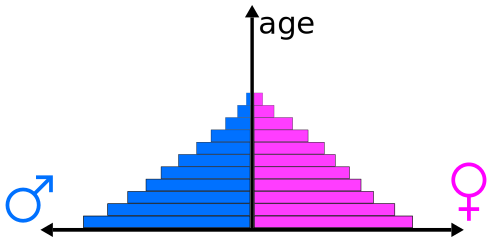
\includegraphics{images/Population_pyramid_example} 

}

\caption{Schematic diagram of a population pyramid (source: Wikipedia)}\label{fig:poppyramid}
\end{figure}

Here we look at the population counts for three countries: Germany,
Mexico and the US from the year 2000. On ELE you will find three files:
``Germanypop.csv'', ``Mexicopop.csv'' and ``USpop.csv'', each with the
following columns:

\begin{itemize}
\tightlist
\item
  \textbf{male}: Population counts for males (\(\times\) 1000);
\item
  \textbf{female}: Population counts for females (\(\times\) 1000).
\end{itemize}

Each row corresponds to an age class, in the order: 0--4, 5--9, 10--14,
15--19, 20--24, 25--29, 30--34, 35--39, 40--44, 45--49, 50--54, 55--59,
60--64, 65--69, 70--74 and 75--79. Mexico then has a final age class of
80+; Germany has final age classes of 80--84 and 85+; and the US has
final age classes of 80--84, 85--89, 90--94 and 90+.

Original source: \href{http://www.census.gov/}{US Census}

(I downloaded these data sets from the very excellent QELP website:
\url{http://www.seattlecentral.edu/qelp/sets/032/032.html}, and wish to
thank the authors for providing a brilliant resource for teaching
statistics.)

In this exercise we will load these data into R, wrangle them into a
useful format and then produce a population pyramid using
\texttt{ggplot2}. We will aim to do all of this using a
\texttt{tidyr}/\texttt{dplyr}/\texttt{ggplot2} workflow where possible.

\section{Data Wrangling}\label{data-wrangling-1}

Firstly, we read the three data files into R, storing them as
\texttt{tbl} objects called \texttt{germany}, \texttt{mexico} and
\texttt{us}, making sure the data frames have informative column names.

\begin{Shaded}
\begin{Highlighting}[]
\NormalTok{## read German data in}
\NormalTok{germany <-}\StringTok{ }\KeywordTok{read.csv}\NormalTok{(}\StringTok{"Germanypop.csv"}\NormalTok{, }\DataTypeTok{header =} \NormalTok{F)}
\NormalTok{## set column names}
\KeywordTok{colnames}\NormalTok{(germany) <-}\StringTok{ }\KeywordTok{c}\NormalTok{(}\StringTok{"male"}\NormalTok{, }\StringTok{"female"}\NormalTok{)}

\NormalTok{## read Mexican data in}
\NormalTok{mexico <-}\StringTok{ }\KeywordTok{read.csv}\NormalTok{(}\StringTok{"Mexicopop.csv"}\NormalTok{, }\DataTypeTok{header =} \NormalTok{F)}
\NormalTok{## set column names}
\KeywordTok{colnames}\NormalTok{(mexico) <-}\StringTok{ }\KeywordTok{c}\NormalTok{(}\StringTok{"male"}\NormalTok{, }\StringTok{"female"}\NormalTok{)}

\NormalTok{## read US data in}
\NormalTok{us <-}\StringTok{ }\KeywordTok{read.csv}\NormalTok{(}\StringTok{"USpop.csv"}\NormalTok{, }\DataTypeTok{header =} \NormalTok{F)}
\NormalTok{## set column names}
\KeywordTok{colnames}\NormalTok{(us) <-}\StringTok{ }\KeywordTok{c}\NormalTok{(}\StringTok{"male"}\NormalTok{, }\StringTok{"female"}\NormalTok{)}

\NormalTok{## produce summaries}
\KeywordTok{summary}\NormalTok{(germany)}
\end{Highlighting}
\end{Shaded}

\begin{verbatim}
##       male          female    
##  Min.   : 339   Min.   :1003  
##  1st Qu.:1960   1st Qu.:2060  
##  Median :2418   Median :2306  
##  Mean   :2247   Mean   :2353  
##  3rd Qu.:2721   3rd Qu.:2774  
##  Max.   :3756   Max.   :3520
\end{verbatim}

\begin{Shaded}
\begin{Highlighting}[]
\KeywordTok{summary}\NormalTok{(mexico)}
\end{Highlighting}
\end{Shaded}

\begin{verbatim}
##       male          female    
##  Min.   : 252   Min.   : 390  
##  1st Qu.:1067   1st Qu.:1200  
##  Median :2383   Median :2742  
##  Mean   :2909   Mean   :2994  
##  3rd Qu.:5060   3rd Qu.:4999  
##  Max.   :5817   Max.   :5580
\end{verbatim}

\begin{Shaded}
\begin{Highlighting}[]
\KeywordTok{summary}\NormalTok{(us)}
\end{Highlighting}
\end{Shaded}

\begin{verbatim}
##       male           female     
##  Min.   :   92   Min.   :  336  
##  1st Qu.: 3683   1st Qu.: 4738  
##  Median : 8662   Median : 8930  
##  Mean   : 6739   Mean   : 7040  
##  3rd Qu.: 9866   3rd Qu.: 9682  
##  Max.   :11231   Max.   :11402
\end{verbatim}

Next we add some information on the age classes. Taking Mexico as an
example, we need to create a \texttt{character} vector containing the
age classes, in the format shown i.e. \texttt{"0-4"} etc. finishing with
\texttt{80+}. Rather than type out the age classes long-hand, we will
start with a \texttt{numeric} vector:
\texttt{age\ \textless{}-\ seq(0,\ 80,\ 5)}, and use various functions
and operators we've already seen to expand this to the format we want:

\begin{Shaded}
\begin{Highlighting}[]
\NormalTok{## set vector of inputs}
\NormalTok{age <-}\StringTok{ }\KeywordTok{seq}\NormalTok{(}\DecValTok{0}\NormalTok{, }\DecValTok{80}\NormalTok{, }\DecValTok{5}\NormalTok{)}

\NormalTok{## create character vector of age classes}
\NormalTok{age <-}\StringTok{ }\KeywordTok{c}\NormalTok{(}
    \KeywordTok{apply}\NormalTok{(}\KeywordTok{cbind}\NormalTok{(age[-}\KeywordTok{length}\NormalTok{(age)], age[-}\DecValTok{1}\NormalTok{] -}\StringTok{ }\DecValTok{1}\NormalTok{), }\DecValTok{1}\NormalTok{, paste, }\DataTypeTok{collapse =} \StringTok{"-"}\NormalTok{),}
    \KeywordTok{paste0}\NormalTok{(age[}\KeywordTok{length}\NormalTok{(age)], }\StringTok{"+"}\NormalTok{))}

\NormalTok{## append age classes}
\NormalTok{mexico <-}\StringTok{ }\KeywordTok{mutate}\NormalTok{(mexico, }\DataTypeTok{age =} \KeywordTok{factor}\NormalTok{(age, }\DataTypeTok{levels =} \NormalTok{age))}

\NormalTok{## tidy up}
\KeywordTok{rm}\NormalTok{(age)}
\end{Highlighting}
\end{Shaded}

\hypertarget{tsk13}{}\bblockT{13}

Go through the code chunk above and make sure you understand what each
component is doing. Try copying-and-pasting discrete parts of the code
to see how these nested functions build up. \eblockT

\hypertarget{tsk14}{}\bblockT{14}

Generate age classes for the German and US datasets, and append an
\texttt{age} column in a similar way. \eblockT

\hyperlink{sol14}{\buttonS{Show Solution}}

This looks good so far; summaries of the three data sets can be seen
below:

\begin{Shaded}
\begin{Highlighting}[]
\KeywordTok{summary}\NormalTok{(germany)}
\end{Highlighting}
\end{Shaded}

\begin{verbatim}
##       male          female          age    
##  Min.   : 339   Min.   :1003   0-4    : 1  
##  1st Qu.:1960   1st Qu.:2060   5-9    : 1  
##  Median :2418   Median :2306   10-14  : 1  
##  Mean   :2247   Mean   :2353   15-19  : 1  
##  3rd Qu.:2721   3rd Qu.:2774   20-24  : 1  
##  Max.   :3756   Max.   :3520   25-29  : 1  
##                                (Other):12
\end{verbatim}

\begin{Shaded}
\begin{Highlighting}[]
\KeywordTok{summary}\NormalTok{(mexico)}
\end{Highlighting}
\end{Shaded}

\begin{verbatim}
##       male          female          age    
##  Min.   : 252   Min.   : 390   0-4    : 1  
##  1st Qu.:1067   1st Qu.:1200   5-9    : 1  
##  Median :2383   Median :2742   10-14  : 1  
##  Mean   :2909   Mean   :2994   15-19  : 1  
##  3rd Qu.:5060   3rd Qu.:4999   20-24  : 1  
##  Max.   :5817   Max.   :5580   25-29  : 1  
##                                (Other):11
\end{verbatim}

\begin{Shaded}
\begin{Highlighting}[]
\KeywordTok{summary}\NormalTok{(us)}
\end{Highlighting}
\end{Shaded}

\begin{verbatim}
##       male           female           age    
##  Min.   :   92   Min.   :  336   0-4    : 1  
##  1st Qu.: 3683   1st Qu.: 4738   5-9    : 1  
##  Median : 8662   Median : 8930   10-14  : 1  
##  Mean   : 6739   Mean   : 7040   15-19  : 1  
##  3rd Qu.: 9866   3rd Qu.: 9682   20-24  : 1  
##  Max.   :11231   Max.   :11402   25-29  : 1  
##                                  (Other):14
\end{verbatim}

One issue is that these three data sets have different age classes. One
way to deal with this is to recategorise the US and German data such
that the top age class is \texttt{80+}. For Germany, this means we have
to sum the entries in the \texttt{80-84} and \texttt{85+} classes, and
for the US it means we have to sum the \texttt{80-84}, \texttt{85-89},
\texttt{90-94} and \texttt{95+} classes. For the German data we can do
something like:

\begin{Shaded}
\begin{Highlighting}[]
\NormalTok{germany <-}\StringTok{ }\NormalTok{germany %>%}
\StringTok{    }\KeywordTok{mutate}\NormalTok{(}\DataTypeTok{age =} \KeywordTok{as.character}\NormalTok{(age)) %>%}\StringTok{ }\NormalTok{## converts factor to character}
\StringTok{    }\KeywordTok{mutate}\NormalTok{(}\DataTypeTok{age =} \KeywordTok{ifelse}\NormalTok{(age ==}\StringTok{ "85+"} \NormalTok{|}\StringTok{ }\NormalTok{age ==}\StringTok{ "80-84"}\NormalTok{, }\StringTok{"80+"}\NormalTok{, age)) %>%}\StringTok{ }\NormalTok{## replaces age categories}
\StringTok{    }\KeywordTok{group_by}\NormalTok{(age) %>%}\StringTok{ }\NormalTok{## groups by age}
\StringTok{    }\KeywordTok{summarise}\NormalTok{(}\DataTypeTok{male =} \KeywordTok{sum}\NormalTok{(male), }\DataTypeTok{female =} \KeywordTok{sum}\NormalTok{(female)) %>%}\StringTok{ }\NormalTok{## sums together counts in additional age groups}
\StringTok{    }\KeywordTok{mutate}\NormalTok{(}\DataTypeTok{age =} \KeywordTok{factor}\NormalTok{(age, }\DataTypeTok{levels =} \KeywordTok{levels}\NormalTok{(mexico$age))) ## converts character back to factor (with correct levels)}
\end{Highlighting}
\end{Shaded}

This first strips the levels information out by converting the
\texttt{age} column to a \texttt{character}. Then we use the
\texttt{ifelse()} function to search-and-replace the relevant strings.
Then we sum together the counts according to different levels of
\texttt{age} (since we now have multiple entries for the \texttt{80+}
age class). Finally we convert \texttt{age} back to a \texttt{factor},
being careful to set the order of the levels to be the same as the
\texttt{mexico} data (remember R converts using lexicographical ordering
otherwise).

\hypertarget{tsk15}{}\bblockT{15}

Run through a similar workflow to recategorise the US age classes.
\eblockT

\hyperlink{sol15}{\buttonS{Show Solution}}

\begin{quote}
\textbf{Note}: a slightly less verbose option would be to use the
\texttt{revalue()} or \texttt{mapvalues()} functions in the
\href{https://cran.r-project.org/web/packages/plyr/}{\texttt{plyr}}
package, see
\href{http://www.cookbook-r.com/Manipulating_data/Recoding_data/}{here}
for some examples.
\end{quote}

Now we will join together the three tables to create one larger data
set. We will first join the three data sets together on the \texttt{age}
column, before gathering together the \texttt{male} and \texttt{female}
counts for each country into two columns, one of population counts
(\texttt{pop}) and one relating to \texttt{sex} (which actually captures
\texttt{sex} and \texttt{country} at this stage). We then separate the
\texttt{sex} and \texttt{country} values into two separate columns,
before setting them to be \texttt{factor} types. We do this using a
single piped workflow that avoids us having to create lots of temporary
objects:

\begin{Shaded}
\begin{Highlighting}[]
\NormalTok{pop <-}\StringTok{ }\NormalTok{germany %>%}
\StringTok{        }\KeywordTok{inner_join}\NormalTok{(mexico, }\StringTok{"age"}\NormalTok{, }\DataTypeTok{suffix =} \KeywordTok{c}\NormalTok{(}\StringTok{"_Germany"}\NormalTok{, }\StringTok{"_Mexico"}\NormalTok{)) %>%}
\StringTok{        }\KeywordTok{inner_join}\NormalTok{(us, }\StringTok{"age"}\NormalTok{) %>%}
\StringTok{        }\KeywordTok{rename}\NormalTok{(}\DataTypeTok{male_US =} \NormalTok{male, }\DataTypeTok{female_US =} \NormalTok{female) %>%}
\StringTok{        }\KeywordTok{gather}\NormalTok{(}\StringTok{"country"}\NormalTok{, }\StringTok{"pop"}\NormalTok{, -age) %>%}
\StringTok{        }\KeywordTok{separate}\NormalTok{(country, }\KeywordTok{c}\NormalTok{(}\StringTok{"sex"}\NormalTok{, }\StringTok{"country"}\NormalTok{), }\DataTypeTok{sep =} \StringTok{"_"}\NormalTok{) %>%}
\StringTok{        }\KeywordTok{mutate}\NormalTok{(}\DataTypeTok{country =} \KeywordTok{factor}\NormalTok{(country), }\DataTypeTok{sex =} \KeywordTok{factor}\NormalTok{(sex))}
\NormalTok{pop}
\end{Highlighting}
\end{Shaded}

\begin{verbatim}
## # A tibble: 102 x 4
##    age   sex   country   pop
##    <fct> <fct> <fct>   <int>
##  1 0-4   male  Germany  2055
##  2 10-14 male  Germany  2458
##  3 15-19 male  Germany  2404
##  4 20-24 male  Germany  2361
##  5 25-29 male  Germany  2623
##  6 30-34 male  Germany  3573
##  7 35-39 male  Germany  3756
##  8 40-44 male  Germany  3263
##  9 45-49 male  Germany  2883
## 10 50-54 male  Germany  2432
## # ... with 92 more rows
\end{verbatim}

\begin{Shaded}
\begin{Highlighting}[]
\KeywordTok{summary}\NormalTok{(pop)}
\end{Highlighting}
\end{Shaded}

\begin{verbatim}
##       age         sex        country        pop       
##  0-4    : 6   female:51   Germany:34   Min.   :  252  
##  5-9    : 6   male  :51   Mexico :34   1st Qu.: 2169  
##  10-14  : 6               US     :34   Median : 3309  
##  15-19  : 6                            Mean   : 4497  
##  20-24  : 6                            3rd Qu.: 5813  
##  25-29  : 6                            Max.   :11402  
##  (Other):66
\end{verbatim}

\hypertarget{tsk16}{}\bblockT{16}

Go through the workflow above and understand what each line is doing and
why. Add comments to the code. If you don't understand, please ask one
of the demonstrators. \eblockT

\section{Visualisation}\label{visualisation}

Finally, we have wrangled our data into a useful form for data analysis.
Now we will try and plot some population pyramids using
\texttt{ggplot2}.

\begin{Shaded}
\begin{Highlighting}[]
\KeywordTok{ggplot}\NormalTok{(pop, }\KeywordTok{aes}\NormalTok{(}\DataTypeTok{x =} \NormalTok{age, }\DataTypeTok{y =} \KeywordTok{ifelse}\NormalTok{(sex ==}\StringTok{ "male"}\NormalTok{, -pop, pop), }\DataTypeTok{fill =} \NormalTok{sex)) +}\StringTok{ }
\StringTok{    }\KeywordTok{geom_bar}\NormalTok{(}\DataTypeTok{stat =} \StringTok{"identity"}\NormalTok{) +}
\StringTok{    }\KeywordTok{scale_y_continuous}\NormalTok{(}\DataTypeTok{breaks =} \KeywordTok{signif}\NormalTok{(}\KeywordTok{seq}\NormalTok{(-}\KeywordTok{max}\NormalTok{(pop$pop), }\KeywordTok{max}\NormalTok{(pop$pop), }\DataTypeTok{length.out =} \DecValTok{5}\NormalTok{), }\DecValTok{2}\NormalTok{), }
                     \DataTypeTok{labels =} \KeywordTok{abs}\NormalTok{(}\KeywordTok{signif}\NormalTok{(}\KeywordTok{seq}\NormalTok{(-}\KeywordTok{max}\NormalTok{(pop$pop), }\KeywordTok{max}\NormalTok{(pop$pop), }\DataTypeTok{length.out =} \DecValTok{5}\NormalTok{), }\DecValTok{2}\NormalTok{))) +}
\StringTok{    }\KeywordTok{coord_flip}\NormalTok{() +}
\StringTok{    }\KeywordTok{facet_wrap}\NormalTok{(~}\StringTok{ }\NormalTok{country, }\DataTypeTok{ncol =} \DecValTok{1}\NormalTok{) +}
\StringTok{    }\KeywordTok{ylab}\NormalTok{(}\StringTok{"Population counts (x1000)"}\NormalTok{) +}
\StringTok{    }\KeywordTok{xlab}\NormalTok{(}\StringTok{"Age (yrs)"}\NormalTok{) +}
\StringTok{    }\KeywordTok{guides}\NormalTok{(}\DataTypeTok{fill =} \KeywordTok{guide_legend}\NormalTok{(}\DataTypeTok{title =} \StringTok{"Sex"}\NormalTok{))}
\end{Highlighting}
\end{Shaded}

\begin{center}\includegraphics{_main_files/figure-latex/unnamed-chunk-107-1} \end{center}

Beautiful isn't it? (The horrendously stereotypical gender colours are
purely a coincidence due to the defaults in \texttt{ggplot2}, please
feel free to change them to something less egregious.) These plots are
hugely informative. We know that countries experiencing fast population
growth typically have a large number of individuals of reproductive age,
with a wider base to the pyramid. In contrast, populations that have
slow, static or even negative growth typically have more older
individuals; their pyramids tend to be wider at the top.

In the year 2000, the population distribution of Mexico shows a very
bottom-heavy pattern, suggesting few older people, but a large number of
young and middle-age people. In fact we can quantify this directly as:

\begin{Shaded}
\begin{Highlighting}[]
\NormalTok{pop %>%}
\StringTok{    }\KeywordTok{group_by}\NormalTok{(country, age) %>%}
\StringTok{    }\KeywordTok{summarise}\NormalTok{(}\DataTypeTok{pop =} \KeywordTok{sum}\NormalTok{(pop)) %>%}
\StringTok{    }\KeywordTok{arrange}\NormalTok{(country, age) %>%}
\StringTok{    }\KeywordTok{group_by}\NormalTok{(country) %>%}
\StringTok{    }\KeywordTok{mutate}\NormalTok{(}\DataTypeTok{cumprop =} \KeywordTok{cumsum}\NormalTok{(pop /}\StringTok{ }\KeywordTok{sum}\NormalTok{(pop))) %>%}
\StringTok{    }\KeywordTok{select}\NormalTok{(-pop) %>%}
\StringTok{    }\KeywordTok{spread}\NormalTok{(age, cumprop)}
\end{Highlighting}
\end{Shaded}

\begin{verbatim}
## # A tibble: 3 x 18
## # Groups:   country [3]
##   country  `0-4`  `5-9` `10-14` `15-19` `20-24` `25-29` `30-34` `35-39`
## * <fct>    <dbl>  <dbl>   <dbl>   <dbl>   <dbl>   <dbl>   <dbl>   <dbl>
## 1 Germany 0.0483 0.0994   0.157   0.214   0.269   0.331   0.415   0.503
## 2 Mexico  0.114  0.227    0.338   0.445   0.545   0.637   0.713   0.777
## 3 US      0.0685 0.140    0.212   0.285   0.352   0.417   0.488   0.569
## # ... with 9 more variables: `40-44` <dbl>, `45-49` <dbl>, `50-54` <dbl>,
## #   `55-59` <dbl>, `60-64` <dbl>, `65-69` <dbl>, `70-74` <dbl>,
## #   `75-79` <dbl>, `80+` <dbl>
\end{verbatim}

\hypertarget{tsk17}{}\bblockT{17}

Go through the workflow above and understand what each line is doing and
why. Add comments to the code. If you don't understand, please ask one
of the demonstrators. \eblockT

We can see here that around 55\% of Mexicans are younger than 25,
compared to around 27\% of Germans and 35\% of Americans. We can also
look at these figures split by sex:

\begin{Shaded}
\begin{Highlighting}[]
\NormalTok{pop %>%}
\StringTok{    }\KeywordTok{arrange}\NormalTok{(country, sex, age) %>%}
\StringTok{    }\KeywordTok{group_by}\NormalTok{(country, sex) %>%}
\StringTok{    }\KeywordTok{mutate}\NormalTok{(}\DataTypeTok{cumprop =} \KeywordTok{cumsum}\NormalTok{(pop /}\StringTok{ }\KeywordTok{sum}\NormalTok{(pop))) %>%}
\StringTok{    }\KeywordTok{select}\NormalTok{(-pop) %>%}
\StringTok{    }\KeywordTok{spread}\NormalTok{(age, cumprop)}
\end{Highlighting}
\end{Shaded}

\begin{verbatim}
## # A tibble: 6 x 19
## # Groups:   country, sex [6]
##   sex    country  `0-4`  `5-9` `10-14` `15-19` `20-24` `25-29` `30-34`
## * <fct>  <fct>    <dbl>  <dbl>   <dbl>   <dbl>   <dbl>   <dbl>   <dbl>
## 1 female Germany 0.0460 0.0946   0.150   0.203   0.257   0.315   0.395
## 2 female Mexico  0.110  0.219    0.327   0.430   0.529   0.619   0.698
## 3 female US      0.0655 0.134    0.203   0.272   0.336   0.400   0.471
## 4 male   Germany 0.0508 0.104    0.165   0.225   0.283   0.348   0.436
## 5 male   Mexico  0.118  0.235    0.350   0.460   0.562   0.654   0.729
## 6 male   US      0.0715 0.147    0.222   0.298   0.369   0.435   0.507
## # ... with 10 more variables: `35-39` <dbl>, `40-44` <dbl>, `45-49` <dbl>,
## #   `50-54` <dbl>, `55-59` <dbl>, `60-64` <dbl>, `65-69` <dbl>,
## #   `70-74` <dbl>, `75-79` <dbl>, `80+` <dbl>
\end{verbatim}

Mexico also has a very high proportion of young females: in fact 33\% of
the current population of women are of pre-reproductive age (0--14
years) and 49\% are of reproductive age (15--44). This means Mexico's
population is expected to rapidly increase in the near future. A general
pattern is that as countries transition from more agricultural economies
to more industrialised economies, birth rates drop (due to better access
to family planning, increased job opportunities for women, and various
other factors). As soon as birth rates approach death rates then
population growth declines, and the population pyramid becomee more
top-heavy. The US is currently classed as a medium-growth country, and
Germany a negative-growth country. The population pyramid plot also
helps visualise the overall differences in population sizes between the
three countries.

A good description of population demographics can be found in this short
video:

Another great site on these sorts of topics is the
\href{https://ourworldindata.org/}{OurWorldInData} project.

\chapter{Answers}\label{answers}

\hypertarget{sol1}{} \bblockS{1}

Eloquent and inspiring solution.

\vspace{\baselineskip}

\hyperlink{tsk1}{\buttonT{Return to task}} \eblockS
\hypertarget{sol2}{} \bblockS{2}

\begin{Shaded}
\begin{Highlighting}[]
\NormalTok{plotGapminder <-}\StringTok{ }\NormalTok{function(data, }\DataTypeTok{year =} \DecValTok{1952}\NormalTok{)}
\NormalTok{\{}
    \NormalTok{## produce point sizes }
    \NormalTok{data$pop <-}\StringTok{ }\NormalTok{data$pop /}\StringTok{ }\KeywordTok{max}\NormalTok{(data$pop)}
    
    \NormalTok{## produce legend sizes}
    \NormalTok{leg_pop <-}\StringTok{ }\KeywordTok{signif}\NormalTok{(}\KeywordTok{quantile}\NormalTok{(data$pop, }\DataTypeTok{probs =} \KeywordTok{c}\NormalTok{(}\FloatTok{0.05}\NormalTok{, }\FloatTok{0.25}\NormalTok{, }\FloatTok{0.5}\NormalTok{, }\FloatTok{0.75}\NormalTok{, }\FloatTok{0.95}\NormalTok{)), }\DecValTok{2}\NormalTok{)}
    \NormalTok{pt_pop <-}\StringTok{ }\KeywordTok{sqrt}\NormalTok{(}\DecValTok{200} \NormalTok{*}\StringTok{ }\NormalTok{leg_pop /}\StringTok{ }\NormalTok{pi)}
    
    \NormalTok{## produce axes ranges}
    \NormalTok{ylims <-}\StringTok{ }\KeywordTok{range}\NormalTok{(data$lifeExp)}
    \NormalTok{xlims <-}\StringTok{ }\KeywordTok{range}\NormalTok{(}\KeywordTok{log10}\NormalTok{(data$gdpPercap))}
    \NormalTok{## extend bounds to fit legend in}
    \NormalTok{ylims[}\DecValTok{1}\NormalTok{] <-}\StringTok{ }\NormalTok{ylims[}\DecValTok{1}\NormalTok{] *}\StringTok{ }\FloatTok{0.9}
    \NormalTok{xlims[}\DecValTok{2}\NormalTok{] <-}\StringTok{ }\NormalTok{xlims[}\DecValTok{2}\NormalTok{] *}\StringTok{ }\FloatTok{1.1}
    
    \NormalTok{## extract subset of data by year}
    \NormalTok{data <-}\StringTok{ }\NormalTok{data[data$year ==}\StringTok{ }\NormalTok{year, ]}
    
    \NormalTok{## produce plot}
    \KeywordTok{plot}\NormalTok{(}\KeywordTok{log10}\NormalTok{(data$gdpPercap), data$lifeExp, }
         \DataTypeTok{pch =} \DecValTok{21}\NormalTok{, }
         \DataTypeTok{bg =} \KeywordTok{as.numeric}\NormalTok{(data$continent),}
         \DataTypeTok{cex =} \KeywordTok{sqrt}\NormalTok{(}\DecValTok{200} \NormalTok{*}\StringTok{ }\NormalTok{data$pop),}
         \DataTypeTok{xlab =} \StringTok{"GDP per capita"}\NormalTok{,}
         \DataTypeTok{ylab =} \StringTok{"Life expectancy at birth (years)"}\NormalTok{,}
         \DataTypeTok{main =} \NormalTok{year,}
         \DataTypeTok{xaxt =} \StringTok{"n"}\NormalTok{,}
         \DataTypeTok{xlim =} \NormalTok{xlims,}
         \DataTypeTok{ylim =} \NormalTok{ylims)}
    \KeywordTok{axis}\NormalTok{(}\DataTypeTok{side =} \DecValTok{1}\NormalTok{, }\DataTypeTok{at =} \DecValTok{3}\NormalTok{:}\DecValTok{5}\NormalTok{, }\DataTypeTok{labels =} \DecValTok{10}\NormalTok{^\{}\DecValTok{3}\NormalTok{:}\DecValTok{5}\NormalTok{\})}
    \KeywordTok{legend}\NormalTok{(}\FloatTok{4.7}\NormalTok{, }\DecValTok{65}\NormalTok{, }\DataTypeTok{legend =} \KeywordTok{levels}\NormalTok{(data$continent), }
           \DataTypeTok{pch =} \DecValTok{21}\NormalTok{, }
           \DataTypeTok{pt.bg =} \DecValTok{1}\NormalTok{:}\KeywordTok{length}\NormalTok{(}\KeywordTok{levels}\NormalTok{(data$continent)),}
           \DataTypeTok{title =} \StringTok{"Continent"}\NormalTok{,}
           \DataTypeTok{bty =} \StringTok{"n"}\NormalTok{)}
    \KeywordTok{legend}\NormalTok{(}\FloatTok{4.7}\NormalTok{, }\DecValTok{43}\NormalTok{, }
           \DataTypeTok{legend =} \NormalTok{leg_pop, }
           \DataTypeTok{pch =} \DecValTok{21}\NormalTok{, }
           \DataTypeTok{pt.cex =} \NormalTok{pt_pop, }
           \DataTypeTok{pt.bg =} \StringTok{"black"}\NormalTok{,}
           \DataTypeTok{title =} \StringTok{"Population size"}\NormalTok{,}
           \DataTypeTok{bty =} \StringTok{"n"}\NormalTok{)}
\NormalTok{\}}
\NormalTok{for(i in }\KeywordTok{c}\NormalTok{(}\DecValTok{1952}\NormalTok{, }\DecValTok{1982}\NormalTok{, }\DecValTok{1992}\NormalTok{, }\DecValTok{2002}\NormalTok{)) \{}
    \KeywordTok{plotGapminder}\NormalTok{(gapminder, i)}
\NormalTok{\}}
\end{Highlighting}
\end{Shaded}

\begin{center}\includegraphics{_main_files/figure-latex/unnamed-chunk-113-1} \end{center}

\begin{center}\includegraphics{_main_files/figure-latex/unnamed-chunk-113-2} \end{center}

\begin{center}\includegraphics{_main_files/figure-latex/unnamed-chunk-113-3} \end{center}

\begin{center}\includegraphics{_main_files/figure-latex/unnamed-chunk-113-4} \end{center}

\vspace{\baselineskip}

\hyperlink{tsk2}{\buttonT{Return to task}} \eblockS
\hypertarget{sol3}{} \bblockS{3}

\begin{Shaded}
\begin{Highlighting}[]
\NormalTok{## change the interval argument to slow animation down}
\KeywordTok{saveGIF}\NormalTok{(\{}
    \NormalTok{## function to produce multiple plots}
    \NormalTok{## which get bound together as a GIF}
    \NormalTok{for(i in }\KeywordTok{sort}\NormalTok{(}\KeywordTok{unique}\NormalTok{(gapminder$year)))\{}
        \KeywordTok{plotGapminder}\NormalTok{(gapminder, i)}
    \NormalTok{\}}
\NormalTok{\}, }\DataTypeTok{movie.name =} \StringTok{"gapminderslow.gif"}\NormalTok{, }
    \DataTypeTok{ani.width =} \DecValTok{500}\NormalTok{, }\DataTypeTok{ani.height =} \DecValTok{500}\NormalTok{,}
    \DataTypeTok{interval =} \DecValTok{1}\NormalTok{)}
\end{Highlighting}
\end{Shaded}

\vspace{\baselineskip}

\hyperlink{tsk3}{\buttonT{Return to task}} \eblockS
\hypertarget{sol4}{} \bblockS{4}

\begin{Shaded}
\begin{Highlighting}[]
\KeywordTok{ggplot}\NormalTok{(gapminder[gapminder$year ==}\StringTok{ }\DecValTok{1952}\NormalTok{, ],}
       \KeywordTok{aes}\NormalTok{(}\DataTypeTok{x =} \NormalTok{gdpPercap, }\DataTypeTok{fill =} \NormalTok{continent)) +}
\StringTok{    }\KeywordTok{geom_histogram}\NormalTok{() +}
\StringTok{    }\KeywordTok{xlab}\NormalTok{(}\StringTok{"GDP per capita"}\NormalTok{) +}\StringTok{ }
\StringTok{    }\KeywordTok{ylab}\NormalTok{(}\StringTok{"Count"}\NormalTok{) +}
\StringTok{    }\KeywordTok{ggtitle}\NormalTok{(}\StringTok{"1952"}\NormalTok{) +}
\StringTok{    }\KeywordTok{guides}\NormalTok{(}\DataTypeTok{fill =} \KeywordTok{guide_legend}\NormalTok{(}\DataTypeTok{title =} \StringTok{"Continent"}\NormalTok{)) }
\end{Highlighting}
\end{Shaded}

\begin{verbatim}
## `stat_bin()` using `bins = 30`. Pick better value with `binwidth`.
\end{verbatim}

\begin{center}\includegraphics{_main_files/figure-latex/unnamed-chunk-115-1} \end{center}

\vspace{\baselineskip}

\hyperlink{tsk4}{\buttonT{Return to task}} \eblockS
\hypertarget{sol5}{} \bblockS{5}

\begin{Shaded}
\begin{Highlighting}[]
\NormalTok{plotGapminder_gg <-}\StringTok{ }\NormalTok{function(data, }\DataTypeTok{year =} \DecValTok{1952}\NormalTok{) \{}
    \NormalTok{p <-}\StringTok{ }\KeywordTok{ggplot}\NormalTok{(gapminder[gapminder$year ==}\StringTok{ }\NormalTok{year, ],}
       \KeywordTok{aes}\NormalTok{(}\DataTypeTok{x =} \NormalTok{gdpPercap, }\DataTypeTok{fill =} \NormalTok{continent)) +}
\StringTok{    }\KeywordTok{geom_histogram}\NormalTok{() +}
\StringTok{    }\KeywordTok{xlab}\NormalTok{(}\StringTok{"GDP per capita"}\NormalTok{) +}\StringTok{ }
\StringTok{    }\KeywordTok{ylab}\NormalTok{(}\StringTok{"Count"}\NormalTok{) +}
\StringTok{    }\KeywordTok{ggtitle}\NormalTok{(year) +}
\StringTok{    }\KeywordTok{guides}\NormalTok{(}\DataTypeTok{fill =} \KeywordTok{guide_legend}\NormalTok{(}\DataTypeTok{title =} \StringTok{"Continent"}\NormalTok{))}
    \KeywordTok{print}\NormalTok{(p)}
\NormalTok{\}}
\NormalTok{for(i in }\KeywordTok{c}\NormalTok{(}\DecValTok{1952}\NormalTok{, }\DecValTok{1982}\NormalTok{, }\DecValTok{1992}\NormalTok{, }\DecValTok{2002}\NormalTok{)) \{}
    \KeywordTok{plotGapminder_gg}\NormalTok{(gapminder, i)}
\NormalTok{\}}
\end{Highlighting}
\end{Shaded}

\begin{verbatim}
## `stat_bin()` using `bins = 30`. Pick better value with `binwidth`.
\end{verbatim}

\begin{center}\includegraphics{_main_files/figure-latex/unnamed-chunk-116-1} \end{center}

\begin{verbatim}
## `stat_bin()` using `bins = 30`. Pick better value with `binwidth`.
\end{verbatim}

\begin{center}\includegraphics{_main_files/figure-latex/unnamed-chunk-116-2} \end{center}

\begin{verbatim}
## `stat_bin()` using `bins = 30`. Pick better value with `binwidth`.
\end{verbatim}

\begin{center}\includegraphics{_main_files/figure-latex/unnamed-chunk-116-3} \end{center}

\begin{verbatim}
## `stat_bin()` using `bins = 30`. Pick better value with `binwidth`.
\end{verbatim}

\begin{center}\includegraphics{_main_files/figure-latex/unnamed-chunk-116-4} \end{center}

\vspace{\baselineskip}

\hyperlink{tsk5}{\buttonT{Return to task}} \eblockS
\hypertarget{sol6}{} \bblockS{6}

\begin{Shaded}
\begin{Highlighting}[]
\NormalTok{## read data into R}
\NormalTok{worms <-}\StringTok{ }\KeywordTok{read.csv}\NormalTok{(}\StringTok{"worms.csv"}\NormalTok{, }\DataTypeTok{header =} \NormalTok{T)}

\NormalTok{## plot histogram for worm density }
\KeywordTok{ggplot}\NormalTok{(worms, }\KeywordTok{aes}\NormalTok{(}\DataTypeTok{x =} \NormalTok{Worm.density)) +}
\StringTok{    }\KeywordTok{geom_histogram}\NormalTok{(}\DataTypeTok{binwidth =} \FloatTok{0.5}\NormalTok{) +}\StringTok{ }
\StringTok{    }\KeywordTok{xlab}\NormalTok{(}\StringTok{"Worm Density"}\NormalTok{)}
\end{Highlighting}
\end{Shaded}

\begin{center}\includegraphics{_main_files/figure-latex/unnamed-chunk-117-1} \end{center}

\begin{Shaded}
\begin{Highlighting}[]
\CommentTok{# plot histogram for area}
\KeywordTok{ggplot}\NormalTok{(worms, }\KeywordTok{aes}\NormalTok{(}\DataTypeTok{x =} \NormalTok{Area)) +}
\StringTok{    }\KeywordTok{geom_histogram}\NormalTok{(}\DataTypeTok{binwidth =} \FloatTok{0.25}\NormalTok{) +}\StringTok{ }
\StringTok{    }\KeywordTok{xlab}\NormalTok{(}\StringTok{"Area"}\NormalTok{)}
\end{Highlighting}
\end{Shaded}

\begin{center}\includegraphics{_main_files/figure-latex/unnamed-chunk-117-2} \end{center}

\begin{Shaded}
\begin{Highlighting}[]
\NormalTok{## box-and-whisker plot for worm density against vegetation}
\KeywordTok{ggplot}\NormalTok{(worms, }\KeywordTok{aes}\NormalTok{(}\DataTypeTok{x =} \NormalTok{Vegetation, }\DataTypeTok{y =}\NormalTok{Worm.density)) +}
\StringTok{    }\KeywordTok{geom_boxplot}\NormalTok{() +}
\StringTok{    }\KeywordTok{ylab}\NormalTok{(}\StringTok{"Worm Density"}\NormalTok{)}
\end{Highlighting}
\end{Shaded}

\begin{center}\includegraphics{_main_files/figure-latex/unnamed-chunk-117-3} \end{center}

\begin{Shaded}
\begin{Highlighting}[]
\NormalTok{## scatter plot for worm density against area with}
\NormalTok{## fitted regression line}
\KeywordTok{ggplot}\NormalTok{(worms, }\KeywordTok{aes}\NormalTok{(}\DataTypeTok{y =} \NormalTok{Worm.density, }\DataTypeTok{x =} \NormalTok{Area)) +}
\StringTok{    }\KeywordTok{geom_point}\NormalTok{() +}
\StringTok{    }\CommentTok{# Add linear regression line}
\StringTok{    }\KeywordTok{geom_smooth}\NormalTok{(}\DataTypeTok{method =} \NormalTok{lm, }\DataTypeTok{se =} \NormalTok{F) +}
\StringTok{    }\KeywordTok{ylab}\NormalTok{(}\StringTok{"Worm Density"}\NormalTok{)}
\end{Highlighting}
\end{Shaded}

\begin{center}\includegraphics{_main_files/figure-latex/unnamed-chunk-117-4} \end{center}

\vspace{\baselineskip}

\hyperlink{tsk6}{\buttonT{Return to task}} \eblockS
\hypertarget{sol7}{} \bblockS{7}

\begin{Shaded}
\begin{Highlighting}[]
\NormalTok{## load data}
\NormalTok{ff <-}\StringTok{ }\KeywordTok{readRDS}\NormalTok{(}\StringTok{"ff.rds"}\NormalTok{)}

\NormalTok{## amend factor labels for type to make}
\NormalTok{## easier to read}
\NormalTok{ff$type <-}\StringTok{ }\KeywordTok{as.character}\NormalTok{(ff$type)}
\NormalTok{ff$type[ff$type ==}\StringTok{ "0"}\NormalTok{] <-}\StringTok{ "Inseminated"}
\NormalTok{ff$type[ff$type ==}\StringTok{ "1"}\NormalTok{] <-}\StringTok{ "Virgin"}
\NormalTok{ff$type[ff$type ==}\StringTok{ "9"}\NormalTok{] <-}\StringTok{ "Control"}
\NormalTok{ff$type <-}\StringTok{ }\KeywordTok{factor}\NormalTok{(ff$type)}

\KeywordTok{ggplot}\NormalTok{(ff, }\KeywordTok{aes}\NormalTok{(}\DataTypeTok{y =} \NormalTok{longevity, }\DataTypeTok{x =} \NormalTok{thorax, }
               \DataTypeTok{colour =} \NormalTok{type)) +}
\StringTok{    }\KeywordTok{geom_point}\NormalTok{() +}
\StringTok{    }\KeywordTok{geom_smooth}\NormalTok{(}\DataTypeTok{method =} \NormalTok{lm, }\DataTypeTok{se =} \NormalTok{F) +}
\StringTok{    }\KeywordTok{facet_wrap}\NormalTok{(~}\StringTok{ }\NormalTok{partners) +}
\StringTok{    }\KeywordTok{guides}\NormalTok{(}\DataTypeTok{colour =} \KeywordTok{guide_legend}\NormalTok{(}\DataTypeTok{title =} \StringTok{"Partner Type"}\NormalTok{)) +}
\StringTok{    }\KeywordTok{ylab}\NormalTok{(}\StringTok{"Longevity (days)"}\NormalTok{) +}
\StringTok{    }\KeywordTok{xlab}\NormalTok{(}\StringTok{"Thorax length (mm)"}\NormalTok{)}
\end{Highlighting}
\end{Shaded}

\begin{center}\includegraphics{_main_files/figure-latex/unnamed-chunk-118-1} \end{center}

\vspace{\baselineskip}

\hyperlink{tsk7}{\buttonT{Return to task}} \eblockS
\hypertarget{sol9}{} \bblockS{9}

\begin{Shaded}
\begin{Highlighting}[]
\NormalTok{gp_hiv <-}\StringTok{ }\KeywordTok{read.csv}\NormalTok{(}\StringTok{"indicator hiv estimated prevalence% 15-49.csv"}\NormalTok{, }\DataTypeTok{header=} \NormalTok{T)}
\NormalTok{gp_hiv <-}\StringTok{ }\NormalTok{gp_hiv %>%}
\StringTok{                }\NormalTok{tbl_df %>%}\StringTok{ }
\StringTok{                }\KeywordTok{gather}\NormalTok{(year, prevalence, -Estimated.HIV.Prevalence.....Ages}\FloatTok{.15.49}\NormalTok{.) %>%}
\StringTok{                }\KeywordTok{mutate}\NormalTok{(}\DataTypeTok{year =} \KeywordTok{as.numeric}\NormalTok{(}\KeywordTok{gsub}\NormalTok{(}\StringTok{"X"}\NormalTok{, }\StringTok{""}\NormalTok{, year))) %>%}
\StringTok{                }\KeywordTok{rename}\NormalTok{(}\DataTypeTok{country =} \NormalTok{Estimated.HIV.Prevalence.....Ages}\FloatTok{.15.49}\NormalTok{.) %>%}
\StringTok{                }\KeywordTok{filter}\NormalTok{(country !=}\StringTok{ ""}\NormalTok{) %>%}
\StringTok{                }\KeywordTok{filter}\NormalTok{(!}\KeywordTok{is.na}\NormalTok{(prevalence)) %>%}
\StringTok{                }\KeywordTok{filter}\NormalTok{(year >}\StringTok{ }\DecValTok{1990}\NormalTok{) %>%}
\StringTok{                }\NormalTok{droplevels}
\end{Highlighting}
\end{Shaded}

\vspace{\baselineskip}

\hyperlink{tsk9}{\buttonT{Return to task}} \eblockS
\hypertarget{sol10}{} \bblockS{10}

\begin{Shaded}
\begin{Highlighting}[]
\NormalTok{## here is one solution using filtering, piping and faceting}
\NormalTok{gp %>%}
\StringTok{    }\KeywordTok{filter}\NormalTok{(year ==}\StringTok{ }\DecValTok{1991} \NormalTok{|}\StringTok{ }\NormalTok{year ==}\StringTok{ }\DecValTok{1997} \NormalTok{|}\StringTok{ }\NormalTok{year ==}\StringTok{ }\DecValTok{2005} \NormalTok{|}\StringTok{ }\NormalTok{year ==}\StringTok{ }\DecValTok{2011}\NormalTok{) %>%}
\StringTok{    }\KeywordTok{mutate}\NormalTok{(}\DataTypeTok{year =} \KeywordTok{factor}\NormalTok{(year)) %>%}
\StringTok{    }\KeywordTok{ggplot}\NormalTok{(}\KeywordTok{aes}\NormalTok{(}\DataTypeTok{x =} \NormalTok{gdp, }\DataTypeTok{y =} \NormalTok{prevalence)) +}
\StringTok{    }\KeywordTok{geom_point}\NormalTok{() +}\StringTok{ }
\StringTok{    }\KeywordTok{scale_x_continuous}\NormalTok{(}\DataTypeTok{trans =} \StringTok{"log10"}\NormalTok{) +}
\StringTok{    }\KeywordTok{xlab}\NormalTok{(}\StringTok{"GDP per capita"}\NormalTok{) +}
\StringTok{    }\KeywordTok{ylab}\NormalTok{(}\StringTok{"HIV prevalence in 15-49 year olds"}\NormalTok{) +}
\StringTok{    }\KeywordTok{facet_wrap}\NormalTok{(~year)}
\end{Highlighting}
\end{Shaded}

\begin{center}\includegraphics{_main_files/figure-latex/unnamed-chunk-120-1} \end{center}

\vspace{\baselineskip}

\hyperlink{tsk10}{\buttonT{Return to task}} \eblockS
\hypertarget{sol11}{} \bblockS{11}

\begin{Shaded}
\begin{Highlighting}[]
\NormalTok{## read in data}
\NormalTok{gp_pop <-}\StringTok{ }\KeywordTok{read.csv}\NormalTok{(}\StringTok{"indicator gapminder population.csv"}\NormalTok{, }\DataTypeTok{header=} \NormalTok{T)}

\NormalTok{## tidy data}
\NormalTok{gp_pop <-}\StringTok{ }\NormalTok{gp_pop %>%}
\StringTok{                }\NormalTok{tbl_df %>%}\StringTok{ }
\StringTok{                }\KeywordTok{gather}\NormalTok{(year, pop, -Total.population) %>%}
\StringTok{                }\KeywordTok{mutate}\NormalTok{(}\DataTypeTok{year =} \KeywordTok{as.numeric}\NormalTok{(}\KeywordTok{gsub}\NormalTok{(}\StringTok{"X"}\NormalTok{, }\StringTok{""}\NormalTok{, year))) %>%}
\StringTok{                }\KeywordTok{rename}\NormalTok{(}\DataTypeTok{country =} \NormalTok{Total.population) %>%}
\StringTok{                }\KeywordTok{filter}\NormalTok{(country !=}\StringTok{ ""}\NormalTok{) %>%}
\StringTok{                }\KeywordTok{filter}\NormalTok{(!}\KeywordTok{is.na}\NormalTok{(pop)) %>%}
\StringTok{                }\KeywordTok{filter}\NormalTok{(year >}\StringTok{ }\DecValTok{1990}\NormalTok{) %>%}
\StringTok{                }\NormalTok{droplevels}

\NormalTok{## check no population data are missing}
\NormalTok{## hence all rows of gp can be matched}
\KeywordTok{anti_join}\NormalTok{(gp, gp_pop, }\DataTypeTok{by =} \KeywordTok{c}\NormalTok{(}\StringTok{"year"}\NormalTok{, }\StringTok{"country"}\NormalTok{))}
\end{Highlighting}
\end{Shaded}

\begin{verbatim}
## Warning: Column `country` joining character vector and factor, coercing
## into character vector
\end{verbatim}

\begin{verbatim}
## # A tibble: 0 x 4
## # ... with 4 variables: country <chr>, year <dbl>, gdp <int>,
## #   prevalence <dbl>
\end{verbatim}

\begin{Shaded}
\begin{Highlighting}[]
\NormalTok{## join to gp table}
\NormalTok{gp <-}\StringTok{ }\KeywordTok{inner_join}\NormalTok{(gp, gp_pop, }\DataTypeTok{by =} \KeywordTok{c}\NormalTok{(}\StringTok{"year"}\NormalTok{, }\StringTok{"country"}\NormalTok{))}
\end{Highlighting}
\end{Shaded}

\begin{verbatim}
## Warning: Column `country` joining character vector and factor, coercing
## into character vector
\end{verbatim}

\vspace{\baselineskip}

\hyperlink{tsk11}{\buttonT{Return to task}} \eblockS
\hypertarget{sol12}{} \bblockS{12}

\begin{Shaded}
\begin{Highlighting}[]
\NormalTok{## here is one solution using filtering, piping and faceting}
\NormalTok{gp %>%}
\StringTok{    }\KeywordTok{filter}\NormalTok{(year ==}\StringTok{ }\DecValTok{1991} \NormalTok{|}\StringTok{ }\NormalTok{year ==}\StringTok{ }\DecValTok{1997} \NormalTok{|}\StringTok{ }\NormalTok{year ==}\StringTok{ }\DecValTok{2005} \NormalTok{|}\StringTok{ }\NormalTok{year ==}\StringTok{ }\DecValTok{2011}\NormalTok{) %>%}
\StringTok{    }\KeywordTok{mutate}\NormalTok{(}\DataTypeTok{year =} \KeywordTok{factor}\NormalTok{(year)) %>%}
\StringTok{    }\KeywordTok{ggplot}\NormalTok{(}\KeywordTok{aes}\NormalTok{(}\DataTypeTok{x =} \NormalTok{gdp, }\DataTypeTok{y =} \NormalTok{prevalence, }\DataTypeTok{size =} \NormalTok{pop)) +}
\StringTok{    }\KeywordTok{geom_point}\NormalTok{() +}\StringTok{ }
\StringTok{    }\KeywordTok{scale_x_continuous}\NormalTok{(}\DataTypeTok{trans =} \StringTok{"log10"}\NormalTok{) +}
\StringTok{    }\KeywordTok{guides}\NormalTok{(}\DataTypeTok{size =} \KeywordTok{guide_legend}\NormalTok{(}\DataTypeTok{title =} \StringTok{"Population size"}\NormalTok{)) +}
\StringTok{    }\KeywordTok{xlab}\NormalTok{(}\StringTok{"GDP per capita"}\NormalTok{) +}
\StringTok{    }\KeywordTok{ylab}\NormalTok{(}\StringTok{"HIV prevalence in 15-49 year olds"}\NormalTok{) +}
\StringTok{    }\KeywordTok{facet_wrap}\NormalTok{(~year)}
\end{Highlighting}
\end{Shaded}

\begin{center}\includegraphics{_main_files/figure-latex/unnamed-chunk-122-1} \end{center}

\vspace{\baselineskip}

\hyperlink{tsk12}{\buttonT{Return to task}} \eblockS
\hypertarget{sol14}{} \bblockS{14}

\begin{Shaded}
\begin{Highlighting}[]
\NormalTok{## append age classes to german data}
\NormalTok{age <-}\StringTok{ }\KeywordTok{seq}\NormalTok{(}\DecValTok{0}\NormalTok{, }\DecValTok{85}\NormalTok{, }\DecValTok{5}\NormalTok{)}
\NormalTok{age <-}\StringTok{ }\KeywordTok{c}\NormalTok{(}
    \KeywordTok{apply}\NormalTok{(}\KeywordTok{cbind}\NormalTok{(age[-}\KeywordTok{length}\NormalTok{(age)], age[-}\DecValTok{1}\NormalTok{] -}\StringTok{ }\DecValTok{1}\NormalTok{), }\DecValTok{1}\NormalTok{, paste, }\DataTypeTok{collapse =} \StringTok{"-"}\NormalTok{),}
    \KeywordTok{paste0}\NormalTok{(age[}\KeywordTok{length}\NormalTok{(age)], }\StringTok{"+"}\NormalTok{))}
\NormalTok{germany <-}\StringTok{ }\KeywordTok{mutate}\NormalTok{(germany, }\DataTypeTok{age =} \KeywordTok{factor}\NormalTok{(age, }\DataTypeTok{levels =} \NormalTok{age))}

\NormalTok{## append age classes to german data}
\NormalTok{age <-}\StringTok{ }\KeywordTok{seq}\NormalTok{(}\DecValTok{0}\NormalTok{, }\DecValTok{95}\NormalTok{, }\DecValTok{5}\NormalTok{)}
\NormalTok{age <-}\StringTok{ }\KeywordTok{c}\NormalTok{(}
    \KeywordTok{apply}\NormalTok{(}\KeywordTok{cbind}\NormalTok{(age[-}\KeywordTok{length}\NormalTok{(age)], age[-}\DecValTok{1}\NormalTok{] -}\StringTok{ }\DecValTok{1}\NormalTok{), }\DecValTok{1}\NormalTok{, paste, }\DataTypeTok{collapse =} \StringTok{"-"}\NormalTok{),}
    \KeywordTok{paste0}\NormalTok{(age[}\KeywordTok{length}\NormalTok{(age)], }\StringTok{"+"}\NormalTok{))}
\NormalTok{us <-}\StringTok{ }\KeywordTok{mutate}\NormalTok{(us, }\DataTypeTok{age =} \KeywordTok{factor}\NormalTok{(age, }\DataTypeTok{levels =} \NormalTok{age))}
\end{Highlighting}
\end{Shaded}

\vspace{\baselineskip}

\hyperlink{tsk14}{\buttonT{Return to task}} \eblockS
\hypertarget{sol15}{} \bblockS{15}

\begin{Shaded}
\begin{Highlighting}[]
\NormalTok{us <-}\StringTok{ }\NormalTok{us %>%}
\StringTok{    }\KeywordTok{mutate}\NormalTok{(}\DataTypeTok{age =} \KeywordTok{as.character}\NormalTok{(age)) %>%}\StringTok{ }\NormalTok{## converts factor to character}
\StringTok{    }\KeywordTok{mutate}\NormalTok{(}\DataTypeTok{age =} \KeywordTok{ifelse}\NormalTok{(age ==}\StringTok{ "95+"} \NormalTok{|}\StringTok{ }\NormalTok{age ==}\StringTok{ "90-94"} \NormalTok{|}\StringTok{ }
\StringTok{                            }\NormalTok{age ==}\StringTok{ "85-89"} \NormalTok{|}\StringTok{ }\NormalTok{age ==}\StringTok{ "80-84"}\NormalTok{, }\StringTok{"80+"}\NormalTok{, age)) %>%}\StringTok{ }\NormalTok{## replaces age categories}
\StringTok{    }\KeywordTok{group_by}\NormalTok{(age) %>%}\StringTok{ }\NormalTok{## groups by age}
\StringTok{    }\KeywordTok{summarise}\NormalTok{(}\DataTypeTok{male =} \KeywordTok{sum}\NormalTok{(male), }\DataTypeTok{female =} \KeywordTok{sum}\NormalTok{(female)) %>%}\StringTok{ }\NormalTok{## sums together counts in additional age groups}
\StringTok{    }\KeywordTok{mutate}\NormalTok{(}\DataTypeTok{age =} \KeywordTok{factor}\NormalTok{(age, }\DataTypeTok{levels =} \KeywordTok{levels}\NormalTok{(mexico$age))) ## converts character back to factor (with correct levels)}
\end{Highlighting}
\end{Shaded}

\vspace{\baselineskip}

\hyperlink{tsk15}{\buttonT{Return to task}} \eblockS

\end{document}
